%!TEX root = main.tex
\chapter{Analyse elliptischer Strukturen mit TAG-Varianten} \label{sec-ellipsenanalyse}


In den beiden vorangegangenen Kapiteln konnte gezeigt werden, dass diskontinuierliche Valenzrealisierungen bei kohärenten Konstruktionen direkt mittels diskontinuierlicher Konstituenten repräsentiert werden können, dass man also die Idealisierung der Kontinuität nicht eingehen muss. In diesem Kapitel werden wir uns der Modellierung unvollständiger Valenzrealisierungen, besser bekannt als \isi{Ellipse} (siehe Kapitel \ref{chap-ellipse}), zuwenden und fragen: Kann die Idealisierung der Vollständigkeit\is{Idealisierung!der Vollständigkeit} ebenso umgangen werden wie die Idealisierung der Kontinuität? Dabei möchte ich analog vorgehen und zunächst in Abschnitt~\ref{sec-ellipsenanalyse-wege} grundsätzliche Modellierungsstrategien unterscheiden, die unabhängig vom gewählten Grammatikformalismus aber mit den jeweils eigenen Mitteln umgesetzt werden können. In den nachfolgenden Abschnitten ruht das Augenmerk wiederum auf TAG-Umsetzungen. 



\section{Modellierungsstrategien} \label{sec-ellipsenanalyse-wege}

Die syntaktische Modellierung elliptischer Strukturen muss sich einer der in Abbildung~\ref{fig-ellipse-strategien} zusammengefassten Modellierungstrategien bedienen:\footnote{Vgl.\ die Taxonomien in \citet[768f,788f]{Klein:93}, \citet[16ff]{Schwabe:94}, \citet[5]{Winkler:Schwabe:03} und \citet[2]{Aelbrecht:10}, die sich in Perspektivierung und Terminologie von der in dieser Arbeit vorgeschlagenen Taxonomie unterscheiden.}
\begin{figure}[t]
\centering
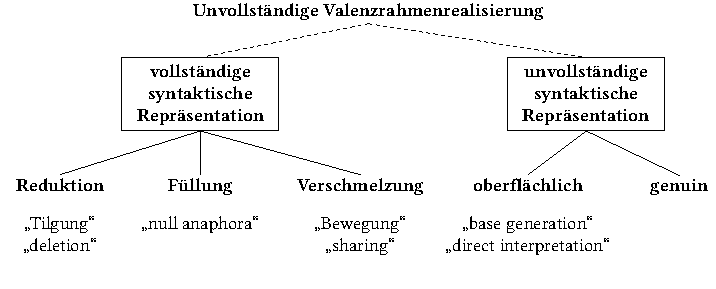
\includegraphics{graphics/abb81.pdf}
\caption{\label{fig-ellipse-strategien}Taxonomie der Modellierungsstrategien bei elliptischen Struk\-turen}
\end{figure}
Entweder ist die syntaktische Repräsentation (in irgendeiner Hinsicht) valenztheoretisch vollständig und die Unvollständigkeit der Oberfläche wird mittels dreier Prozesse erklärt, die ich hier Verschmelzung, Reduktion und Füllung nennen möchte; oder die syntaktische Repräsentation ist, genau wie die Oberfläche, valenztheoretisch unvollständig.

\subsubsection*{Reduktion}\is{Reduktion|(}

Unter \textsc{Reduktion} fallen solche Verfahren, bei denen die syntaktische Repräsentation $R_v$ eines Valenzrahmens $v$ so gestutzt wird, dass die resultierende syntaktische Repräsentation $R_v'$ der Oberflächenrealisierung von $v$ entspricht. Um dies zu veranschaulichen, betrachten wir nochmals das Gapping-Datum in \ref{ex-koord-6-a} auf Seite \pageref{ex-koord-6-a}, hier wiederholt in \ref{ex-ellipsenanalyse-1}:

\ex.  \label{ex-ellipsenanalyse-1}\ldots [$\kappa_2$ der Tourist \sout{sah} drei Waschbären]

Unter dem Blickwinkel der Reduktion ist hier das finite Verb als Teil einer Substruktur aus der syntaktischen Repräsentation entfernt worden. Die betroffene Substruktur kann unterschiedlich gro\ss\ sein (vom Terminal bis zum Teilbaum) und nur bestimmte syntaktische Repräsentationsebenen betreffen. Ein bekanntes Beispiel für Letzteres ist die Reduktion auf der phonetischen Form (PF)\is{phonetische Form (PF)}, die im Rahmen der Generativen Grammatik\is{Generative Grammatik} vorgeschlagen wurde (siehe z.\,B.\ \citealt{Klein:93}; \citealt{Hartmann:00}; \citealt{Merchant:01}) und mittlerweile einer Reduktion auf der "`syntaktischen Struktur"' (D-Struktur/S-Struktur) vorgezogen wird.
\is{Reduktion|)}

\subsubsection*{Füllung}\is{Füllung|(}

Spiegelbildlich zur Reduktion verhält sich die \textsc{Füllung}: Die syntaktische Repräsentation wird nicht gestutzt, sondern mit opakem Material bzw.\ "`leeren Kategorien"'\is{leere Kategorie} aufgefüllt. \citet[98f]{Wasow:72} stellt diesen Ansatz im Rahmen der generativen Grammatik als \isi{Empty Structures Hypothesis (ESH)} vor und bezeichnet die leeren Terminale als Null-Anaphern\is{Null-Anapher} ("`null anaphors"'), die er mit dem  $\Delta$-Symbol markiert.\footnote{Siehe auch \cite{Wasow:79}. Eine aktuellere Arbeit dieser Art liefert beispielsweise \cite{Johnson:01}.} In \ref{ex-ellipseanalyse-esh} markiert das $\Delta$-Symbol die Füllung des finiten Verbs:
\largerpage% 

\ex. [$\kappa_1$ Der Jäger sah einen Hasen] und [$\kappa_2$ der Tourist $\Delta$ drei Waschbären].\label{ex-ellipseanalyse-esh}

Wasow nimmt im Rahmen der ESH an, dass Füllungen (bzw.\ Null-Anaphern) strukturiert\is{Füllung!strukturierte} sind, mehr noch, dass eine phrasenstrukturelle Isomorphie zwischen Ellipse und \isi{Antezedens} besteht: "`null anaphors have all the structure of their antecedents, lacking only phonetic material"' \citep[98]{Wasow:72}. Komplexe Ellipsen werden also mit mehreren Null-Anaphern, d.\,h.\ $\Delta$, gefüllt und phrasenstrukturell gegliedert. Die Sätze in \ref{ex-fuellung-2} veranschaulichen die ESH anhand einer VP-Ellipse\is{Ellipse!VP-}, eines Sluicing-Falls\is{Ellipse!Sluicing} und eines Gapping-Falls\is{Ellipse!Gapping}, wobei die zugrunde gelegte Phrasenstruktur der Lesbarkeit halber ohne Phrasenmarker angezeigt wird:

\largerpage%  

\ex. \label{ex-fuellung-2}
\a. John heard someone out back, but he doesn't know [who [$\Delta$ [$\Delta$ $\Delta$]]]. %\hfill \citep{???}
\b. John will come to the party if Mary can [$\Delta$ [$\Delta$ [$\Delta$]]].\\
\citep[(31)]{Wasow:72}
\c. I want to try to begin to write a novel, and Mary [$\Delta$ [$\Delta$ [$\Delta$ [$\Delta$  a play]]]].\label{ex-fuellung-2-c}

Die Einschätzung von \citet[6]{Winkler:Schwabe:03}, dass es sich bei dieser Art des Füllungsansatzes (bzw.\ "`interpretive position"') um einen Vorläufer der \isi{PF-Tilgung} handelt, ist ohne Schwierigkeiten nachvollziehbar. 
 
Es ist jedoch auch denkbar, dass Füllungen\is{Füllung!unstrukturierte} phrasenstrukturell vom \isi{Antezedens} abweichen. Dies ist Grundlage der sogenannten \isi{Non-Expansion Hypothesis (NEH)}, erstmals wohl in \cite{Akmajian:68} formuliert,\footnote{Siehe \citet[94]{Wasow:72}: "`This approach, to be referred to as the non-expansion hypothesis, asserts that every phonetically anaphor consists simply of a dummy symbol (say $\Delta$) which is associated by interpretive rules with an antecedent."' Leider wurde \cite{Akmajian:68} nie veröffentlicht und ich konnte kein Exemplar ausfindig machen.} nach der die Füllungen (bzw.\ Null-Anaphern\is{Null-Anapher}) keinerlei interne Struktur besitzen. Statt einer Vielzahl von Füllungen wird den Sätze in \ref{ex-fuellung-2} nun genau eine atomare Füllung zugesprochen: 

\ex. \label{ex-fuellung-3}
\a. \label{ex-fuellung-3-a}John heard someone out back, but he doesn't know who $\Delta$.
\b. \label{ex-fuellung-3-b}John will come to the party if Mary can $\Delta$.
\c. \label{ex-fuellung-3-c}I want to try to begin to write a novel, and Mary $\Delta$ a play.

Die NEH\is{Non-Expansion Hypothesis (NEH)} stie\ss\ wegen dieser atomaren Füllungen bereits bei \cite{Ross:69} auf Ablehnung, u.\,a.\ mit dem Argument, dass sie damit die \isi{Kasusmarkierung} gesluicter\is{Ellipse!Sluicing} \textit{Wh}-Pronomen nicht erklären könne.\footnote{\cite{Ross:69} richtet seine Kritik nicht direkt auf einen Füllungsansatz mit unstrukturierten Null-Anaphora\is{Non-Expansion Hypothesis (NEH)}, sondern auf eine (damals noch nicht vorgebrachte) Sluicing-Analyse\is{Ellipse!Sluicing}, bei der das gesluicte \textit{Wh}-Pronomen kein Überbleibsel eines \textit{Wh}-Gliedsatzes bildet. Direkt betroffen ist etwa der Ansatz von \cite{Riemsdijk:78} und auch die Ansätze mit freistehenden Phrasen bzw.\ phrasalen Äu\ss erungen (siehe S.\,\pageref{ex-freistehende-phrasen}). Es ist wohl \cite{Wasow:72}, der einen Bezug zwischen Ross' Kritik und unstrukturierten Null-Anaphern herstellt. Trotzdem wurden unstrukturierte Füllungen z.\,B.\ von \cite{Chung:etal:95} für die Sluicing-Modellierung propagiert. } Dieses Argument ist allerdings abhängig von der Prämisse, dass Kasusrektion durch die Phrasenstruktur bestimmt wird. Ich möchte auf diese Kritik und ihre Voraussetzungen nicht genauer eingehen, denn mir geht es hier in erster Linie um Aspekte der Ellipsenmodellierung. 
 
Wie diese Füllung rekonstruiert\is{Rekonstruktion} wird, ob durch syntaktische (z.\,B.\ \citealt{Fiengo:May:94,Chung:etal:95}), semantische (z.\,B.\ \citealt{Dalrymple:etal:91}) oder diskurs"=basierte (z.\,B.\ \citealt{Hardt:93,Hardt:99,Hardt:Romero:04}) Identität mit einem Antezedens, ist ein ganz anderes Problemfeld.\footnote{Siehe z.\,B.\ \citet[Kapitel~3]{Schlangen:03} für eine Übersicht.} Zunächst einmal liegt hier eine reguläre, voll ausgeprägte syntaktische Struktur vor -- mit dem gravierendem Zugeständnis allerdings, dass manche Terminale "`unsichtbar"' oder phonetisch leer sind. Im Ergebnis ähnelt diese Modellierungstrategie daher stark der phonetischen \isi{Reduktion} in \ref{ex-ellipsenanalyse-1}. Es gibt allerdings auch deutliche Unterschiede: Das leere Terminal ist nicht Ergebnis eines nachgeordneten phonetischen Prozesses, sondern Bestandteil des Lexikons, worin es per se nur sehr rudimentäre Spezifizierungen morphosyntaktischer und semantischer Natur mit sich führt. Das PF-reduzierte Material erscheint dagegen bis auf die phonologische Information voll ausspezifiziert. 

Die Ähnlichkeiten und Unterschiede zwischen Reduktions- und Füllungsansätzen erklären sich meiner Ansicht nach mit deren unterschiedlichen Perspektive auf elliptische Strukturen. Während bei der Reduktion eine Sprachgenerierungsperspektive eingenommen wird, herrscht bei der Füllung eine Sprachverarbeitungsperspektive vor.
\is{Füllung|)}

\subsubsection*{Verschmelzung}\is{Verschmelzung|(}

Im Unterschied zur Reduktion und Füllung wird bei der \textsc{Verschmelzung} die Stipulierung elliptischer Strukturen vermieden: Zwei distinkte syntaktische Repräsentationen unterschiedlicher Valenzrahmenrealisierungen werden hier so zusammengefügt, dass sie gemeinsame Bestandteile besitzen. Das Resultat kann man beispielsweise in \ref{ex-ellipsenanalyse-2} mit einer Bewegungsmetapher\is{Bewegung} veranschaulichen: 

\ex. \label{ex-ellipsenanalyse-2} Heute$_i$ sah$_j$ [$\kappa_1$ $t_i$ $t_j$ der Jäger einen Hasen] und [$\kappa_2$ $t_i$ $t_j$ der Tourist drei Waschbären]. 

\largerpage%
Die Satzglieder {\it heute} und {\it sah} werden aus den Konjunkten herausbewegt und dabei verschmolzen. Da die Konjunkte gleicherma\ss en betroffen sind, spricht man in Anlehnung an \cite{Williams:78,Williams:81} von Across-the-Board-Bewegung (ATB-Bewegung)\is{Bewegung!Across-the-Board}. Einen Verschmelzungsansatz ohne Bewegungskonzept findet man dagegen in Arbeiten zur \isi{Dependenzgrammatik} (z.\,B.\ \citealt{Hudson:88,Pickering:Barry:93}), in deren Augen der Satz \ref{ex-ellipsenanalyse-2} wohl eine Dependenzstruktur\is{Dependenzgraph} wie in \ref{ex-ellipsenanalyse-3} erhalten würde:\footnote{Die Idee des Across-the-Board\is{Bewegung!Across-the-Board} ("`any dependency relation which crosses a conjunct boundary must be shared by all the conjuncts"', \citealt[323]{Hudson:88}) wird Hudson zufolge durch sein \isi{DICS-Prinzip} (siehe Abschnitt~\ref{sec-koordinationsellipsen-5}) erfasst.}
%\largerpage%

\vspace{6ex}

\ex. \scalebox{0.95}{\label{ex-ellipsenanalyse-3} \rnode[t]{1}{Heute} \rnode[t]{2}{sah} [$\kappa_1$ \rnode[t]{3}{der Jäger} \rnode[t]{4}{einen Hasen}] und [$\kappa_2$ \rnode[t]{5}{der Tourist} \rnode[t]{6}{drei Waschbären}].}
\ncarc[offset=0pt,ncurv=1.5,nodesepA=1pt,nodesepB=3pt,arcangleA=-90,arcangleB=-85]{->}{2}{1}
\ncarc[offset=0pt,ncurv=1,nodesepA=1pt,nodesepB=3pt,arcangleA=90,arcangleB=90]{->}{2}{3}
\ncarc[offset=0pt,nodesepA=1pt,nodesepB=3pt,arcangleA=90,arcangleB=90]{->}{2}{4}
\ncarc[offset=0pt,ncurv=0.45,nodesepA=1pt,nodesepB=3pt,arcangleA=90,arcangleB=90]{->}{2}{5}
\ncarc[offset=0pt,ncurv=0.4,nodesepA=1pt,nodesepB=3pt,arcangleA=90,arcangleB=90]{->}{2}{6}

\largerpage[1.7]
Das finite Verb {\it sah} ist hier der gemeinsame Regent der Konjunktkonstituenten. Da ihm in diesem Fall, entsprechend der $\kappa$-Instanziierung als Konstituentenkoordination\is{Koordination!Konstituenten-}, eine Position au\ss erhalb der Konjunkte zugewiesen werden kann, spricht \cite{Osborne:08} von Conjunct-External Sharing. Verschmelzungsprozesse werden jedoch nicht nur bei Konstituentenkoordination angenommen, sondern auch  bei eindeutigen Fällen der Satzkoordination\is{Koordination!Satz-}, wie etwa dem Gapping-Datum\is{Ellipse!Gapping} in \ref{ex-ellipsenanalyse-4}:  

\vspace{5ex}

\ex.\label{ex-ellipsenanalyse-4} [$\kappa_1$ \rnode{1}{der Jäger} \rnode{2}{sah} \rnode{3}{einen Hasen}] und [$\kappa_2$ \rnode{4}{der Tourist} \rnode{5}{drei Waschbären}].
\ncarc[offset=0pt,ncurv=1.2,nodesepA=1pt,nodesepB=3pt,arcangleA=-90,arcangleB=-85]{->}{2}{1}
\ncarc[offset=0pt,ncurv=1,nodesepA=1pt,nodesepB=3pt,arcangleA=90,arcangleB=90]{->}{2}{3}
\ncarc[offset=0pt,ncurv=0.5,nodesepA=1pt,nodesepB=3pt,arcangleA=90,arcangleB=90]{->}{2}{4}
\ncarc[offset=0pt,ncurv=0.4,nodesepA=1pt,nodesepB=3pt,arcangleA=90,arcangleB=90]{->}{2}{5}

Osborne nennt diesen Sharingtyp folgerichtig Conjunct-Internal Sharing. Und auch die ATB-Bewegung\is{Bewegung!Across-the-Board} kann auf Gapping-Daten angewandt werden, wenn man wie \cite{Johnson:04,Johnson:09} ein Bewegungsmuster wie in \ref{ex-ellipsenanalyse-5} annimmt:

\ex. \label{ex-ellipsenanalyse-5} Der Jäger$_i$ sah$_j$ [$\kappa_1$ $t_i$ $t_j$ einen Hasen] und [$\kappa_2$ der Tourist $t_j$ drei Waschbären].

Die Eigenart dieses Bewegungsmusters und der entscheidende Unterschied zum Bewegungsmuster in \ref{ex-ellipsenanalyse-2} oben ist die asymmetrische Entleerung der Konjunkte, denn aus dem ersten Konjunkt wird nicht nur das finite Verb {\it sah} (im Gleichschritt mit dem zweiten Konjunkt) herausbewegt, sondern auch das \isi{Subjekt} {\it der Jäger}. Letztere Bewegung verstö\ss t eigentlich gegen Ross' \isi{Coordinate Structure Constraint} \citep[161]{Ross:67}. 
  
Ein anderer Verschmelzungsansatz für Konstituentenstrukturen, der syntaktische Strukturen mit multipler Dominanz und kreuzenden Kanten\is{kreuzende Kante} vorsieht, wird z.\,B.\ in \cite{McCawley:82} und \cite{Wilder:99,Wilder:08} vorgeschlagen. Dort erhalten Gapping-Daten\is{Ellipse!Gapping} eine syntaktische Struktur wie in Abbildung~\ref{fig-ellipse-verschmelzung}, in der der präterminale V-Knoten des geteilten finiten Verbs von den VP-Knoten beider Konjunkte dominiert wird. 

\clearpage 
 
\begin{figure}[t]
\centering
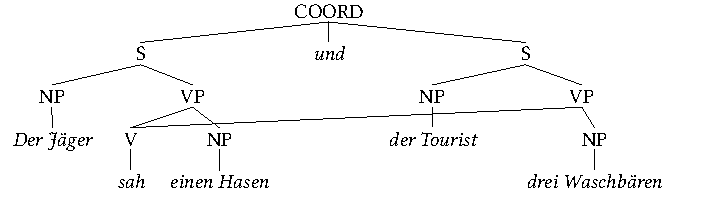
\includegraphics{graphics/abb82.pdf}
\caption{\label{fig-ellipse-verschmelzung}Gapping-Modellierung mit multipler Dominanz und kreuzenden Kanten}
\end{figure} 
 
Auch der CCG-Ansatz\is{Combinatorial Categorial Grammar (CCG)} aus \cite{Steedman:90} bedient sich meiner Meinung nach der Verschmelzungsstrategie. Abbildung~\ref{fig-ellipse-ccg} zeigt die CCG-Ableitung einer Gapping"=Konstruktion\is{Ellipse!Gapping} (zusammengesetzt aus (63) und (85) in \citealt{Steedman:90}). 
\begin{figure}[t]
\centering
\newcommand{\ccghspc}{-0.7em} 
\scalebox{0.81}{
\hspace{-0.5em}
\deriv{8}{
\cmc{2}{\mathrm{Harry ~~ eats ~~ beans}} & & \mathrm{and} & \mathrm{Barry}   & & \mathrm{potatoes} & \\
 \bareline{2} & & \bareline{1} & \bareline{1}  & \hspace{-1em}_{\ftr}  & \bareline{1} & \hspace{-1.2em}_{\btr} \\
 \cmc{2}{\mathit{S}} & & \mathit{conj} & \mathit{S/(S\bs NP)} & & \mathit{(S\bs NP)\bs ((S\bs NP)/NP)} \\
 \bareline{2} & \hspace{-0.8em}_{<dec} & \bareline{2} & \hspace{-0.8em}_{>\&} \\
 (S\bs NP)/NP & S\bs((S\bs NP)/NP) & & \cmc{2}{[S/(S\bs NP)]_\&} \\
 & & & \bareline{4} & \hspace{-0.8em}_{\fbx{}} \\
 & & & \cmc{4}{[S\bs ((S\bs NP)/NP)]_\&} \\
 & \cmc{6}{\hrulefill_{<\&}}  \\
 & \cmc{6}{S\bs ((S\bs NP)/NP)} \\
\cmc{6}{\hrulefill_{<}} \\
\cmc{6}{S} 
}
}
\caption{\label{fig-ellipse-ccg}CCG-Ableitung einer Gapping-Konstruktion aus \citet[(63),(85)]{Steedman:90}}
\end{figure}
Durch eine Reihe von Ableitungsschritten, auf die ich hier nicht detailliert eingehen möchte, erhält das zweite Konjunkt die komplexe Kategorie $[S\bs ((S\bs$""$\mathit{NP})/\mathit{NP})]_\&$. Das zweite Konjunkt bedarf also der funktionalen Applikation mit etwas von der Kategorie $(S\bs NP)/NP$, z.\,B.\ ein Verb mit zwei NP"=Komplementen, um die $S$-Kategorie ableiten zu können. Da die (hier stark vereinfachte) Koordinationsregel $X ~ X \Rightarrow X$ für beliebige Kategorie $X$ ein erstes Konjunkt derselben Kategorie verlangt, steht die CCG-Ableitung zunächst vor einem Problem: Das erste Konjunkt ist nämlich ein vollständiger Satz, also von der Kategorie $S$, und eine Anwendung der Koordinationsregel nicht möglich. Steedmans Ausweg besteht darin, die $S$-Kategorie zu dekomponieren (mittels $dec(ompose)$-Regel bzw.\ "`Left Conjunct Revealing Rule"') und durch zwei andere Kategorien zu ersetzen: $(S\bs NP)/NP$ und $S\bs((S\bs NP)/NP)$. Die erste Kategorie entspricht wieder der Kategorie eines Verbs mit zwei NP"=Komplementen, die zweite Kategorie ist dagegen die des zweiten Konjunkts. Der Anwendung der Koordinationsregel und einer anschlie\ss enden funktionalen Applikation zur Ableitung der $S$-Kategorie steht dann nichts mehr im Wege. Von einer Verschmelzung kann hier deswegen gesprochen werden, weil das Verb durch die $dec$-Regel quasi herausgelöst und mit beiden Konjunkten verrechnet wird. Das Verb des ersten Konjunkts ist also auch das Verb des zweiten Konjunkts. 

All diese Verschmelzungsansätze vermeiden zwar die Stipulation elliptischer Strukturen, sie können aber auch nur dort eingesetzt werden, wo sich zwei Valenzrahmenrealisierungen satzintern finden lassen. Das ist im Rahmen einer \isi{Koordination} vertretbar, bei Adjazenzellipsen\is{Ellipse!Adjazenz-} jedoch schon fragwürdig und bei freien Ellipsen\is{Ellipse!ohne Antezedens} schlie\ss lich ausgeschlossen.
\is{Verschmelzung|)}

\subsubsection*{Unvollständige syntaktische Repräsentation}\is{Unvollständigkeit|(}  

Soweit die Modellierungsstrategien unter dem Vorsatz einer vollständigen syntaktischen Repräsentation von Valenzrahmen. Naturgemä\ss\ unterscheiden sich diese erheblich von Modellierungsansätzen, die nicht von einer so beschaffenen Vollständigkeit ausgehen, deren Repräsentationen man eine Unvollständigkeit prima facie also nicht ansieht. Beim Gapping\is{Ellipse!Gapping} beispielsweise wird dann auf die direkte Repräsentation des fehlenden finiten Verbs verzichtet, was einer Baumstruktur wie in Abbildung~\ref{fig-ellipse-unvollstaendig} entspricht.
\begin{figure}[t]
\centering
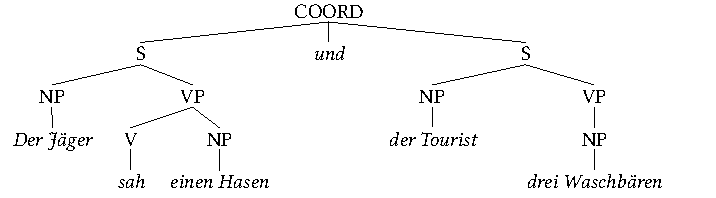
\includegraphics{graphics/abb83.pdf}
\caption{\label{fig-ellipse-unvollstaendig}Basisgenerierung einer Gapping-Struktur}
\end{figure}
Da diese Baumstruktur quasi direkt generiert wird, d.\,h.\ ohne nachfolgende Tilgung, nennt \cite{Chao:87} diesen Ansatz "`base generation"' und schlägt (im Rahmen der Prinzipien-und-Parameter-Theorie) ein "`defektes"' \isi{X-bar-Schema} vor, das sogenannte H\~{}"=Schema, welches Phrasenstrukturregeln der Form IP\~{}$\to$ NP, IP\~{}$\to$ NP I\~{} oder IP\~{}$\to$ I\~{} erlaubt. Damit ist es also möglich, Projektionen\is{Projektion} ohne \isi{Kopf} ("`H\textasciitilde-projections"') zu generieren, wobei die Projektionsstufen mit einer Tilde markiert sind. Die naheliegende Anwendungsdomäne für H\~{}-Strukturen sind Fälle von Gappping, wohingegen Chao bei VPE und Sluicing eine Modellierung mittels H$^{+}$-Strukturen wählt.\footnote{Subjektlücken behandelt \cite{Chao:87} nicht.} Solche "`eigenen syntaktischen Regeln"' \citep[789]{Klein:93} scheinen zumindest in diesem grammatiktheoretischen Kontext, in dem das Verb als Keimzelle der Satzprojektion verstanden wird, unvermeidlich zu sein. 

Chaos Arbeit gilt zwar als wichtiger Bezugspunkt des Forschungsdiskurses, ihr Ansatz wurde jedoch meines Wissens nach nicht entsprechend weiterverfolgt. Als Ausnahme müssen \cite{Culicover:Jackendoff:05} gelten, auch wenn ihre Arbeit eine radikale Weiterentwicklung ("`Simpler Syntax"') der traditionellen \isi{Generative Grammatik}, der Chaos Ansatz verpflichtet ist, darstellt. Sie nehmen für die Ellipsemodellierung ebenfalls spezielle kopflose Phrasenstrukturen an, für Gapping\is{Ellipse!Gapping} beispielsweise die \isi{Phrasenstruktur} in \ref{ex-tag-unvoll-3}:\footnote{Die Phrasenstruktur in \ref{ex-tag-unvoll-3} ist Instanziierung einer allgemeineren Gappingregel \citep[276]{Culicover:Jackendoff:05}, die auch für freistehendes Gapping gilt. Die Überbleibsel freistehender Ellipsen sind jedoch unmittelbare Konstitutenten einer syntaktischen Entität der Kategorie U(tterance) \citep[237f]{Culicover:Jackendoff:05}. U kann auch S einbetten, jedoch nicht umgekehrt.}

\ex. \label{ex-tag-unvoll-3}[$_S$ NP$^{\mathit{ORPH}_1}$ NP$^{\mathit{ORPH}_2}$]$^{\mathit{IL}}$ \hfill \citep[277]{Culicover:Jackendoff:05}

Die $ORPH$-Superskripte markieren Konstituenten, die zusammen mit der unvollständigen S-Phrase einer indirekten Lizenzierung ($IL$) durch das Antezedens bedürfen. Im Gegensatz zur Rezeptionssituation im Rahmen der Generativen Grammatik gibt es im Rahmen der HPSG\is{Head-driven Phrase Structure Grammar (HPSG)} eine Reihe von Arbeiten (z.\,B.\ \citealt{Ginzburg:Sag:01}; \citealt[333f]{Ginzburg:Cooper:04}; \citealt[171ff]{Schlangen:03}), die solche "`defekten"' Strukturen bei der Modellierung elliptischer Antworten\is{Frage-Antwort-Folge} einsetzen. 

Der Basisgenerierungsansatz mittels "`defekter"' Strukturen muss trotz gewisser Ähnlichkeiten von bestimmten Modellierungsansätzen unterschieden werden, die sich mit "`non-senten\-tial utterances"', also mit freien Ellipsen\is{Ellipse!ohne Antezedens} mit nur einem Überbleibsel, befassen. In Arbeiten wie \cite{Yanofsky:78}, \cite{Barton:90} und zuletzt in Arbeiten von Robert Stainton, etwa \cite{Stainton:98,Stainton:06}, werden sie nicht als Sätze analysiert, sondern als freistehende Phrasen, d.\,h.\ als NPs, APs, VPs etc.:

\ex. \label{ex-freistehende-phrasen}
A: He might be moving up to the major leagues soon. \\
B: Never. \newline
[$_{\mathit{ADV}\,''}$ [$_{\mathit{ADV}\,'}$ [$_{\mathit{ADV}}$ never]]] \\
\citep[60]{Barton:90}
 
\newpage
In dieselbe Kerbe schlägt auch \citet[233ff]{Riemsdijk:78} bei seiner Sluicing-Analyse\is{Ellipse!Sluicing}. Diese freistehenden Phrasen sind an sich vollständig -- und damit sind solche Ansätze eigentlich für unsere Darstellung der Modellierungsstrategien für elliptische Strukturen irrelevant. Hier findet zwar wie bei \cite{Chao:87} keine Reduktion, Verschmelzung oder Füllung statt, aber es sind eben auch keine "`eigenen syntaktischen Regeln"' notwendig, d.\,h.\ es müssen keine wesentlichen Änderungen am \isi{X-bar-Schema} und der \isi{Phrasenstruktur} vorgenommen werden.\footnote{Die einzige Änderung laut \citet[53ff]{Barton:90} ist die Erweiterung der Menge der Startsymbole um "`major lexical categories"', kurz $X^{max}$, worin u.\,a.\ N'', P'', ADV'' und V'' enthalten sind.} Was Chaos Ansatz und die Annahme von freistehende Phrasen jedoch zweifellos gemeinsam haben, ist die Herausforderung, die \isi{Kasusmarkierung} ganz anders herzuleiten als sonst üblich, nämlich nicht über die Kasusrektion durch das regierende Verb. Dieses fehlt ja in beiden Fällen in der syntaktischen Repräsentation. Darüber hinaus vereint \cite{Merchant:04} (in einer kritischen Auseinandersetzung) beide Ansätze unter dem Begriff der "`direct interpretation"', da die semantische Komposition ebenfalls neue Wege beschreiten muss, d.\,h.\ nicht über eine vollständige, wenn auch reduzierte oder gefüllte syntaktische Struktur geleitet werden kann.\footnote{Merchant drückt es folgenderma\ss en aus: "`we must allow non-sentential objects either to be able to denote propositions, or we must allow the non-propositional semantic objects to which they give rise to be able to be used to make assertions (further, under some assumptions, we may also need to propose new ways of building syntactic structures)."' \citep[662]{Merchant:04}} 

Die genannten Ansätze, die unvollständige syntaktische Repräsentationen mittels "`defekter"' Strukturen basisgenerieren, werde ich unten in Abschnitt~\ref{sec-unvollständige-repräsentation} als \textsc{oberflächlich unvollständig}\is{Unvollständigkeit!oberflächliche} klassifizieren und \textsc{genuin unvollständigen Ansätzen}\is{Unvollständigkeit!genuine} gegenüberstellen. Letztere generieren unvollständige syntaktische Repräsentationen ohne Rückgriff auf "`eigene syntaktischen Regeln"'.\is{Unvollständigkeit|)} %\\


Damit sind nun also die Modellierungsstrategien für elliptische Strukturen kurz dargestellt worden. Im Folgenden gehe ich auf diejenigen Umsetzungen genauer ein, die im Rahmen von TAG\is{Tree Adjoining Grammar (TAG)} vorgeschlagen wurden -- zunächst auf Verschmelzungsansätze, da es sich bei diesen um die ersten und bis heute prominentesten Versuche handelt, elliptische Strukturen mittels TAG zu modellieren. Angesichts vielfältiger Schwierigkeiten dieser Verschmelzungsansätze werde ich mich für das TT-MCTAG-Modell jedoch einer Reduktions- bzw.\ Füllungsstrategie bedienen und sie in den darauf folgenden Abschnitten ausarbeiten. Daran schlie\ss en sich Bemerkungen zur Basisgenerierung von Ellipsen an, die in das nächste Kapitel überleiten.    


\section{Verschmelzung}

Die Verschmelzungsstrategie\is{Verschmelzung} wurde bisher in zwei sehr unterschiedlichen Ansätzen für das TAG-Framework aufgegriffen: Der eine Ansatz nimmt eine Verschmelzung von Elementarbäumen vor, während der andere Ansatz Ellipse und Antezdens in einer elementaren Baummenge bündelt. Beide Ansätze setzen jedoch die Verfügbarkeit eines Antezedens voraus, weswegen sie für die Modellierung freier Ellipsen ungeeignet sind. 

\subsection{Verschmelzung von Elementarbaumknoten}\is{Kontraktion|(}

Anoop Sarkar und Aravind Joshi schlagen in \cite{Sarkar:Joshi:96,Sarkar:Joshi:97} die Hinzunahme einer weiteren Verknüpfungsoperation {\tt conjoin} vor, die die Verschmelzung oder \isi{Kontraktion} ("`contraction"') von nicht-terminalen Blättern der Konjunkte und damit ein "`sharing of arguments"' erlaubt.\footnote{Erste Ideen für diesen Ansatz finden sich bereits in \cite{Joshi:Schabes:91}. \cite{Chen-Main:06} wendet den Kontraktionsansatz auch bei \textit{Wh}-Bewegung an. Sie plädiert für die Verwendung mehrwurzliger Graphen bei der Repräsentation syntaktischer Strukturen.} Sie demonstrieren ihre Vorgehensweise an folgendem englischen Satz mit Subjektlücke\is{Ellipse!Subjektlücke}:

\ex. \label{ex-contraction-1} Chapman eats cookies and \sout{Chapman} drinks beer.\\
\citep[(7)]{Sarkar:Joshi:97}

Ausgangspunkt für die Derivation von \ref{ex-contraction-1} sind die üblichen Elementarbäume für die Verben {\it eats} und {\it drinks} und ein Elementarbaum für den Konjunktor ("`coordination schema"'), die in Abbildung~\ref{fig-contraction-1} dargestellt werden.
\begin{figure}[t]
\centering
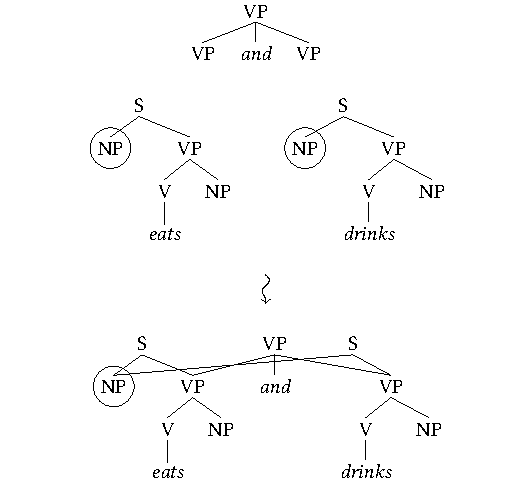
\includegraphics{graphics/abb85.pdf}
\caption{\label{fig-contraction-1}Ableitung von \ref{ex-contraction-1} in der Kontraktionanalyse (vgl.\ \citealt[Abbildung~7]{Sarkar:Joshi:97})}
\end{figure}
Die durch die {\tt conjoin}-Operation aus diesen Elementarbäumen resultierende Struktur ist kein Baum, sondern ein Graph mit Multidominanz und kreuzenden Kanten\is{kreuzende Kante}. Und auch die Ableitungsstruktur ist ein mehrwurzliger Graph, da die Substitution an einem kontrahierten Blatt auf beide kontrahierten Elementarbäume bezogen wird (mutatis mutandis mit Adjunktion und Fu\ss knoten). {\tt Chapman} substituiert quasi gleichzeitig in {\tt eats} und {\tt drinks} jeweils an der Gorn-Adresse 1 und die Ableitungsstruktur sieht deshalb so aus wie in Abbildung~\ref{fig-contraction-2}.

\begin{figure}[t]
\centering
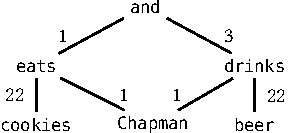
\includegraphics{graphics/abb86.pdf}
\caption{\label{fig-contraction-2}Mehrwurzliger Ableitungsgraph für die Ableitung in Abbildung~\ref{fig-contraction-1}}
\end{figure}

Solche Strukturen weichen gravierend von den üblichen Baumstrukturen des TAG-Frameworks\is{Tree Adjoining Grammar (TAG)} und von klassischen Konstituentenstrukturen allgemein ab. Das kann trotzdem verschmerzbar sein, wenn dadurch linguistische und computationelle Kernprinzipien nicht bedroht sind. Ein Gefühl des Unwohlseins bleibt indessen. \cite{Sarkar:Joshi:97} skizzieren deswegen einen Weg, aus den abgeleiteten Graphen Baumstrukturen zu rekonstruieren, indem Kanten umgehängt und vereinigt werden. Auf diese Weise kann beispielsweise aus dem Graphen in Abbildung~\ref{fig-contraction-1} der abgeleitete Baum in Abbildung~\ref{fig-kontraktion-baumisierung} (vgl.\ \citealt[Abbildung~16]{Sarkar:Joshi:97}) gewonnen werden. Das funktioniert in diesem Fall, weil eine VP-Koordination\is{Koordination!VP-} vorliegt. Bei Fällen der RNR"=Koordination und des Gappings sind die kreuzenden Kanten dagegen nicht auf diese Weise eliminierbar. 

\begin{figure}[t]
\centering
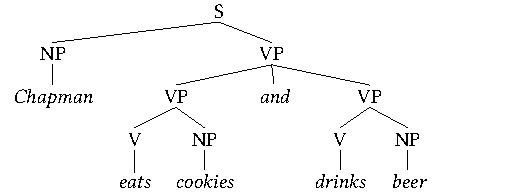
\includegraphics{graphics/abb87.pdf}
\caption{\label{fig-kontraktion-baumisierung}Abgeleiteter Baum für \ref{ex-contraction-1}, der aus dem abgeleiteten Graphen in Abbildung~\ref{fig-contraction-1} konstruiert ist}
\end{figure}

Soweit die Idee der \isi{Kontraktion}. Eine Spezifizierung der {\tt conjoin}-Operation muss auf die folgenden Fragen eine Antwort geben: Welche Knoten können kontrahieren? Wo befindet sich der Yield des kontrahierten Knotens? Mit welchen Knoten der Konjunktbäume wird der Elementarbaum des Konjunktors verknüpft? \cite{Sarkar:Joshi:96,Sarkar:Joshi:97} beantworten dies ungefähr so: 

\begin{enumerate}
  \item Zwei Knoten können kontrahieren, falls sie (i) Blätter sind und (ii) ein identisches Label und (iii) eine identische \isi{Gorn-Adresse} bezüglich des Elementarbaums besitzen.
  \item Was die Lokalisierungsregeln für kontrahierte Knoten betrifft, äußern sich Sarkar und Joshi leider nur sehr vage. Ich konkretisiere ihre Andeutungen folgenderma\ss en: Entsteht ein Knoten $v_k$ durch die Kontraktion der Knoten $v_1$, $v_2$, dann übernimmt $v_k$ die Position von $v_1$ oder $v_2$. Au\ss erdem muss die lineare Präzedens aus den Elementarbäumen beibehalten werden, um ungrammatische Sätze wie \ref{ex-ellipse-12} zu verhindern.

\ex.\label{ex-ellipse-12}
\a. *Eats cookies and Chapman drinks beer.
\b. *Keats steals apples and Chapman eats.

Die relative lineare Ordnung von Schwesterknoten muss also beibehalten werden. 
\item Die Konjunktbäume ersetzen die Blätter des Konjunktorbaums ähnlich wie bei der Substitution, mit dem Unterschied allerdings, dass mehrwurzlige Resultate erlaubt sind, dass also nicht nur der Wurzelknoten, sondern im Prinzip jeder Knoten des Konjunktbaums als Verknüpfungspunkt dienen kann. Der Verknüpfungspunkt im Konjunktbaum wird durch den Algorithmus {\tt FindRoot} bestimmt, der denjenigen Knoten auswählt, der alle nicht-kontrahierten Blätter minimal dominiert. 
\end{enumerate} 

Mit dieser Spezifizierung der {\tt conjoin}-Operation ist es jedoch nicht möglich, selbst einfache Fälle von Gapping\is{Ellipse!Gapping} wie in \ref{ex-contraction-2} abzuleiten:

\ex. \label{ex-contraction-2}John ate bananas and Bill strawberries. 

Zum einen scheitert das daran, dass dafür Präterminale der lexikalischen Anker kontrahiert werden müssen, die per definitionem keine Blätter eines Elementarbaums sind. Sarkar und Joshi schlagen deshalb vor, die Elementarbäume in unlexikalisiertem Zustand zu verwenden. Die Lexikalisierung ("`lexical insertion"') ist also ein nachgeordneter Prozess, vergleichbar mit Substitution und Adjunktion, und der unlexikalisierte Elementarbaum um das benötigte Blatt reicher. Dadurch können mit der {\tt conjoin}-Operation Graphen mit kontrahierten, unlexikalisierten V-Knoten wie in Abbildung~\ref{fig-contraction-3} erzeugt werden, die im Weiteren u.\,a.\ für die Ableitung von \ref{ex-contraction-2} benötigt werden. Man beachte, dass dieses {\tt conjoin}-Resultat mit der Lokalisierungsregel vereinbar ist, die ich oben angegeben habe.

\begin{figure}[t]
\centering
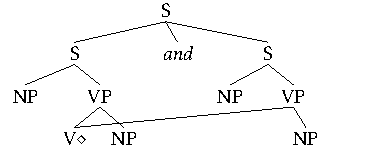
\includegraphics{graphics/abb88.pdf}
\caption{\label{fig-contraction-3}Ergebnis der Kontraktion von V-Knoten in unlexikalisierten Elementar\-bäumen}
\end{figure}

Was passiert aber, wenn wir komplexere Gappingfälle\is{Ellipse!Gapping} betrachten? Sarkar und Joshi behaupten nämlich, ohne das beispielhaft auszuführen, dass auch Sätze wie \ref{ex-contraction-3} durch {\tt conjoin} erfasst werden können:

\ex. \label{ex-contraction-3}John wants Penn to win and Bill \sout{wants} Princeton \sout{to win}. 

Wenn wir die unlexikalisierten Elementarbäume für {\it wants} und {\it to win} in Abbildung~\ref{fig-contraction-4} zugrunde legen, ist es unvermeidbar, dass {\tt conjoin} nicht nur auf unlexikalisierte Elementarbäume, sondern auch auf abgeleitete Bäume anzuwenden ist.\footnote{Dazu hei\ss t es in \citet[21]{Sarkar:Joshi:97} lapidar: "`lexical insertion has to be handled by the parser while building a derivation."'} Der Grund dafür ist, dass die zu kontrahierenden Blätter aus unterschiedlichen Elementarbäumen stammen und die {\tt conjoin}-Operation letztlich auf das ganze Konjunkt bezogen wird und nicht nur auf Elementarbäume.
\begin{figure}[t]
\centering
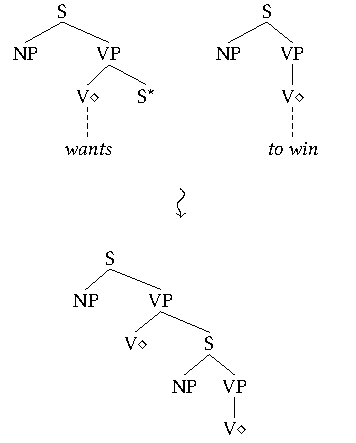
\includegraphics{graphics/abb89.pdf}
\caption{\label{fig-contraction-4}Erzeugung eines unlexikalisierten abgeleiteten Baums für die darauf folgende Kontraktionsanalyse des komplexen Gappingdatums in \ref{ex-contraction-3}}
\end{figure}
Mit anderen Worten: {\tt conjoin} kann zu einem beliebigen Zeitpunkt der Ableitung ausgeführt werden. Die im Zusammenhang mit einfachem Gapping in Abbildung~\ref{fig-contraction-4} beobachtete Reihenfolge von {\tt conjoin}, Lexikalisierung, Adjunktion und Substitution stellt also nur eine von mehreren Möglichkeiten dar.%\\  

Zum Abschluss der Darstellung des Kontraktionsansatzes möchte ich noch auf zwei Probleme hinweisen. Erstens sind durchaus Formen der RNR"=Koordination\is{Koordination!Right-Node-Raising} denkbar, die die Kontraktion von Knoten erfordern, die keine identischen Gorn-Adressen\is{Gorn-Adresse} besitzen. Satz \ref{ex-contraction-4} liefert ein Beispiel dafür:  

\ex. \label{ex-contraction-4} Peter gives him, but Susi eats the cookies.

{\it gives} ist ein ditransitives Verb, {\it eats} dagegen ein transitives Verb. Wenn man, wie \citet[Abbildung~20]{Sarkar:Joshi:97}, für {\it gives} den Elementarbaum in Abbildung~\ref{fig-contraction-5} annimmt, muss das geteilte Objekt {\it the cookies} in den Elementarbäumen der beiden Verben eine unterschiedliche Gorn-Adresse besitzen (hier 23 versus 22).
\begin{figure}[t]
\centering
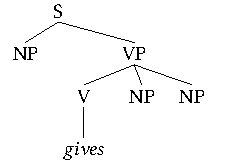
\includegraphics{graphics/abb810.pdf}
\caption{\label{fig-contraction-5}Elementarbaum für das ditransitive Verb {\it gives}}
\end{figure}
Diese Situation lässt sich zwar mit der Wahl eines anderen Elementarbaums vermeiden, es zeigt jedoch, dass der Kontraktionsansatz spürbaren Einfluss auf die Struktur der Elementarbäume hat. %Ähnliches lässt sich allerdings auch vom Reduktionsansatz behaupten.

\newpage
Es ist zweitens unklar, welche Komplexitätseigenschaft diese TAG-Erweiter\-ungen haben. Im Rahmen der XTAG-Implementierung\is{XTAG} \citep{xtag:01} wird die Integration dieses Ansatzes wegen des Auf"|tretens gravierender Parsingambiguitäten als schwierig dargestellt und für einen späteren Zeitpunkt versprochen.\footnote{"`It is important to say that this implementation of predicative coordination is not part of the XTAG release at the moment due massive parsing ambiguities. This is partly because of the current implementation and also the inherent ambiguities due to VP coordination that cause a combinatorial explosion of the parser. We are trying to remedy both of these limitations using a probability model for coordination attachments which will be included as part of a later XTAG release."' \citep[224]{xtag:01}} Wenn ich mit meiner Vermutung hinsichtlich der Kontraktionsanalyse komplexer Gappingfälle Recht habe, dann muss die Abfolge von lexikalischer Ankerung, Kontraktion, Substitution und Adjunktion im Derivationsprozess im Prinzip unbestimmt sein. Das führt aber dann dazu, dass das Lexikon, d.\,h.\ die Menge der lexikalisierten Bäume, nicht nur unendlich gro\ss, sondern auch unendlich ambig ist: Manche verbalen Anker wie etwa {\it wants}, das in VP-übergreifenden Gappingfällen partizipieren kann, lexikalisieren eine unendlich gro\ss e Menge von Baumschablonen. Dieses Ausma\ss\ an Ambiguität tritt übrigens auch dann auf, wenn Koordinationen\is{Koordination} mit beliebig vielen Konjunkten modelliert werden sollen. Aus komplexitätstheoretischer Sicht ist das sicherlich unerwünscht.    
\is{Kontraktion|(}


\subsection{Verschmelzung durch Bündelung in Baummengen}

Djam\'e Seddah und Kollegen schlagen in \cite{Seddah:08} und \cite{Seddah:etal:10} eine Modellierung verschiedener Formen der Koordinationsellipsen mit Hilfe von Baummengen vor, d.\,h.\ im Rahmen einer MCTAG\is{Multi-Component TAG (MCTAG)}. Ihren Ausgangspunkt hat der MCTAG-Ansatz zwar in \cite{Seddah:Sagot:06}, genauer betrachtet handelt es sich dort aber um einen Füllungsansatz, der LTAG verwendet, und auf den ich deshalb im nächsten Abschnitt eingehe.

Die Idee des MCTAG-Ansatzes ist die Bündelung von Ellipse und Antezedens in einer elementaren Baummenge. Dementsprechend werden zur Gappingmodellierung\is{Ellipse!Gapping} elementare Baummengen angenommen, die die Elementarbäume des ellidierten Verbs und des Antezedensverbs enthalten. \cite{Seddah:etal:10} demonstrieren diese Vorgehensweise anhand der Modellierung von Satz \ref{ex-seddah-1} in Abbildung~\ref{fig-seddah-1}:

\ex. \label{ex-seddah-1} Jean aime$_i$ Marie et Paul $\varepsilon_i$ Virginie. \hfill \citep[(1)]{Seddah:etal:10}

Der Elementarbaum des ellidierten Verbs wird durch ein phonetisch leeres Terminal\is{leere Kategorie} $\varepsilon$ lexikalisiert, der abgesehen davon den Valenzrahmen von {\it aime} realisiert. Seddah und Kollegen nennen solche Bäume "`ghost trees"'. Diese Baummenge kann baumlokal\is{Multi-Component TAG (MCTAG)!baumlokale (TL-MCTAG)} mit dem Konjunktorbaum verknüpft werden. Im Unterschied zur Kontraktionsanalyse\is{Kontraktion} kommt also keine neuartige Verknüpfungsoperation zum Einsatz und es werden auch keine kreuzenden Kanten im abgeleiteten Baum und Ableitungsbaum erzeugt. Dafür muss z.\,B.\ in Kauf genommen werden, dass der valenztheoretische Status dieser Baummengen fragwürdig ist. Die Baummenge in Abbildung~\ref{fig-seddah-1} repräsentiert nämlich mehrere Instanzen des {\it aime}-Valenzrahmens. 

\begin{figure}[t]
\centering
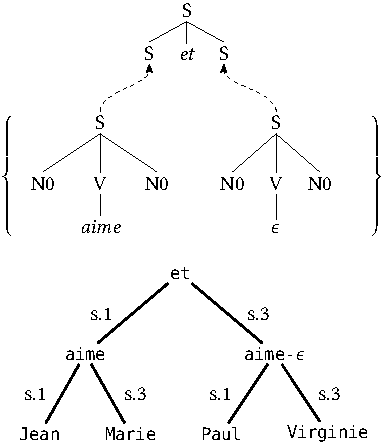
\includegraphics{graphics/abb811.pdf}
\caption{\label{fig-seddah-1}Ableitung der Gappingkonstruktion in \ref{ex-seddah-1} mittels Ellipse-Antezedens-Bündelung (vgl.\ \citealt[Abbildung~1]{Seddah:etal:10})}
\end {figure}


Analog dazu können Ellipse und Antezedens wie in Abbildung~\ref{fig-seddah-rnr} gebündelt werden, um etwa die RNR-Konstruktion\is{Koordination!Right-Node-Raising} in \ref{ex-seddah-rnr} zu modellieren:  

\ex. \label{ex-seddah-rnr}  Marie fabrique $\varepsilon_i$ et Pierre vend des cr\^{e}pes$_i$. \hfill \citep[(2)]{Seddah:etal:10}

\begin{figure}[t]
\centering
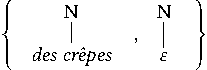
\includegraphics{graphics/abb812.pdf}
\caption{\label{fig-seddah-rnr}Bündelung von Antezedens- und Ellipsenbaum für die nominale Ergänzung {\it des cr\^{e}pes}}
\end{figure}    
Ob auch diese Baummenge baumlokal\is{Multi-Component TAG (MCTAG)!baumlokale (TL-MCTAG)} verwendet wird, ist abhängig von der Modellierung der \isi{Koordination}. Drei Möglichkeiten sind denkbar: (i) Die Konjunkte, d.\,h.\ die Valenzrahmen des jeweiligen maximal übergeordneten Verbs,  und der Konjunktor werden in einem Elementarbaum repräsentiert; dann genügt Baumlokalität. (ii) Die Konjunkte und der Konjunktor werden als separate Elementarbäume repräsentiert, wobei die Konjunkte die Elemente einer Baummenge bilden; dann wird zumindest Mengenlokalität\is{Multi-Component TAG (MCTAG)!mengenlokale (SL-MCTAG)} benötigt. (iii) Die Konjunkte werden als separate Elementarbäume repräsentiert, ohne in einer Baummenge gebündelt zu sein; dann wird Nicht-Lokalität\is{Multi-Component TAG (MCTAG)!nichtlokale (NL-MCTAG)} benötigt. In \citet[Abbildung~2]{Seddah:etal:10} wird die zweite Möglichkeit verfolgt und mit der Baummenge in Abbildung~\ref{fig-seddah-rnr-2} gearbeitet. (Zur Bedeutung der sekundären Kanten kommen wir gleich.) Das ist valenztheoretisch jedoch mindestens ebenso problematisch wie die Ellipse-Antezedens-Bündelung beim Gapping, denn hier sind sogar unterschiedlich geankerte Elementarbäume und damit gänzlich distinkte Valenzrahmen in einer Baummenge enthalten.    

\cite{Seddah:etal:10} beschreiben noch einen weiteren Ansatz zur Modellierung von Ergänzungsellipsen, der keine Ellipse-Antezedens-Bündelung der Ergänzung gebraucht, dafür allerdings eine Erweiterung von MCTAG einführt. Die Idee besteht darin, die Substitutionsknoten der verbalen Valenzrahmen in Abbildung~\ref{fig-seddah-rnr-2} mit sekundären gerichteten Kanten zu verbinden, durch die ein potentielles Sharing-Verhältnis spezifiziert werden kann. Seddah und Kollegen nennen diese Erweiterung "`MCTAG with Local Shared Derivations"' (MCTAG-LSD): Wenn zwei Knoten $v_1$, $v_2$  zweier Elementarbäume $\gamma_1$, $\gamma_2$ durch eine Sharing-Kante $\langle v_1,v_2 \rangle$ verbunden sind, dann substituiert in $v_1$ ein vollwertiger Initialbaum $\alpha$, während in $v_2$ ein "`ghost tree"' $\alpha_\varepsilon$ substituiert werden kann. $\alpha$ und $\alpha_\varepsilon$ müssen jedoch nicht Schwesterelemente einer Baummenge sein. Schlie\ss lich wird der Ableitungsbaum so angepasst, dass $\gamma_2$ nicht $\alpha_\varepsilon$ dominiert, sondern $\alpha$. In Abbildung~\ref{fig-seddah-rnr-2} ist diese Form der Ableitung für die RNR-Koordination\is{Koordination!Right-Node-Raising} in \ref{ex-seddah-rnr}  durchgespielt. 

\begin{figure}[t]
\centering
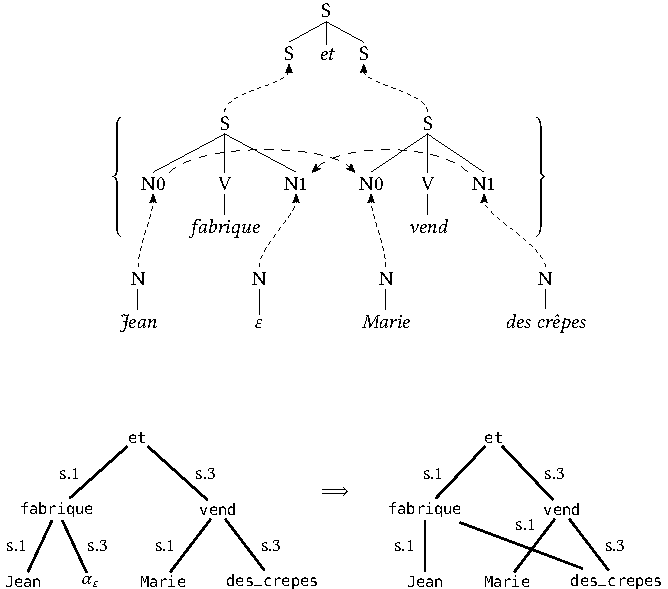
\includegraphics{graphics/abb813.pdf}
\caption{\label{fig-seddah-rnr-2}Ableitung von \ref{ex-seddah-rnr} im Bündelungsansatz mit sekundären Kanten (vgl.\ \citealt[Abbildung~2]{Seddah:etal:10})}
\end{figure}
   
\largerpage
Aus meiner Sicht sind die Sharing-Links nicht unbedingt notwendig, um die Verwendung der "`ghost trees"' zu kontrollieren. Hierfür würden wohl passend gewählte Knoten-Merkmale ausreichen. Seddah und Kollegen geht es hier vor allem um die Überwindung der bekannten Diskrepanz zwischen Ableitungsstruktur und Dependenzstruktur\is{Dependenzgraph}.\footnote{\cite{Seddah:etal:10} gehen deshalb auch auf Kontrollkonstruktionen\is{Kontrolle} ein und nehmen Bezug auf die Vorarbeit von \cite{Seddah:Gaiffe:05}, in der der "`ghost tree"' (bzw.\ ein fehlender Argumentbaum bei einer "`incomplete derivation"', \citealt[292]{Seddah:Gaiffe:05}) als Trigger für eine Fusionsoperation auf dem Ableitungsbaum verstanden wird. Diese Fusionsoperation wird in \cite{Seddah:Sagot:06} zwar auf die Ellipsemodellierung übertragen, aber erst in \cite{Seddah:08} und \cite{Seddah:etal:10} mit einer MCTAG kombiniert, um bestimmte Gappingphänomene ("`zeugma construction"') erfassen zu können. Da ich in \cite{Seddah:Sagot:06} einen Füllungsansatz erkenne, komme ich darauf in Abschnitt~\ref{sec-fuellung} zu sprechen.} 

%\clearpage  

Wenn man die Vorschläge von \cite{Seddah:etal:10} auf die MCTAG"=Modellierung ohne Local Shared Derivation reduziert, d.\,h.\ ohne nachträgliche Anpassungen des Ableitungsbaums, dann ist der Eindruck zwiespältig: Zwar werden keine neuartigen Verknüpfungsoperationen benötigt und keine irregulären Strukturen erzeugt, anders als beispielsweise im Kontraktionsansatz\is{Kontraktion} von \cite{Sarkar:Joshi:97}, aber die Elementarstrukturen fassen mehrere Valenzrahmen zusammen. Die Folge  ist nicht nur, dass das Valenzprinzip\is{Wohlgeformtheitsprinzip!Valenzprinzip} au\ss er Kraft gesetzt werden muss, sondern auch, dass das Lexikon um eine nicht unwesentliche Anzahl von Elementarstrukturen vergrö\ss ert wird. Betrachtet man Koordinationen\is{Koordination} mit beliebig vielen Konjunkten, dann führt dieser Ansatz tatsächlich zu einem unendlich gro\ss en und unendlich ambigen Lexikon -- darin vergleichbar dem Kontraktionsansatz.\footnote{Um Koordinationen mit beliebig vielen Konjunkten in einer Elementarstruktur zu repräsentieren, bedienen sich \cite{Seddah:etal:10} einer Faktorisierung mittels der Kleene-Operatoren * und +. Dieses Vorgehen ist bereits aus Schema-TAG \citep{Harbusch:00b} bekannt.}    



\section{Reduktion} \label{sec-deanchoring}

In Anbetracht der vielfältigen Probleme von Verschmelzungsansätzen im TAG-Framework schlage ich zusammen mit Laura Kallmeyer in \cite{Lichte:Kallmeyer:10} ein Reduktionsverfahren\is{Reduktion} vor. 

\subsection{Entankerung im Ableitungsbaum}

Einer Idee aus \cite{Kobele:09} für Minimalist Gram\-mar\is{Minimalist Grammar} folgend, ist der Ansatzpunkt hier nicht der abgeleitete Baum, sondern der \isi{Ableitungsbaum}: Knoten im Ableitungsbaum können abhängig von internen und externen Bedingungen einer \textsc{Entankerung}\is{Entankerung} ("`de-anchoring"') unterzogen werden, d.\,h.\ die lexikalischen Anker des dazugehörigen Elementarbaums werden getilgt oder durch das leere Terminal\is{leere Kategorie} $\varepsilon$ ersetzt. Dies entspricht der Idee klassischer PF-Tilgungs-Ansätze\is{PF-Tilgung} und führt zu einer strukturellen Isomorphie von \isi{Ellipse} und \isi{Antezedens}. \cite{Lichte:Kallmeyer:10} veranschaulichen die Ent\-anker\-ungs\-idee anhand des Gapping-Datums in \ref{ex-deanchoring-1}: 

\ex. \label{ex-deanchoring-1} Adam praised Mary, and Peter \sout{praised} the waitress.   
  
Zunächst wird das zweite Konjunkt regulär mittels der Elementarbäume in Abbildung~\ref{fig-deanchoring-1} deriviert und in einem zweiten Schritt der \isi{Wurzelknoten} des Ableitungsbaums\is{Ableitungsbaum} entankert. Der entankerte Ableitungsbaum wird so wie in Abbildung~\ref{fig-deanchoring-2} mit durchgestrichenem Knotenlabel dargestellt. 

\begin{figure}[t]
\centering
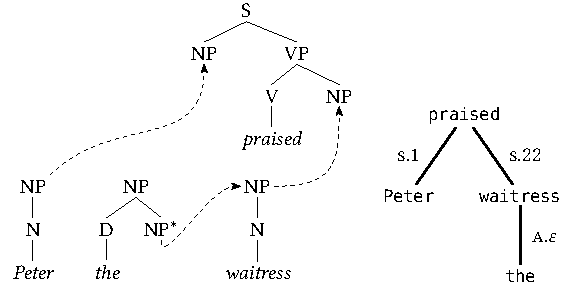
\includegraphics{graphics/abb814.pdf}
\caption{\label{fig-deanchoring-1}Ableitung und Ableitungsbaum für "`Peter praised the waitress"' \citep[Abbildung~4]{Lichte:Kallmeyer:10}}
\end{figure}
 

\begin{figure}[t]
\centering
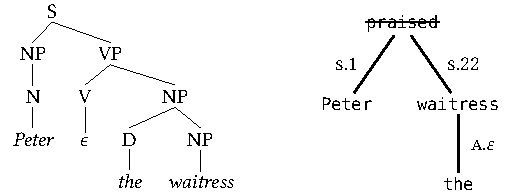
\includegraphics{graphics/abb815.pdf}
\caption{\label{fig-deanchoring-2}Abgeleiteter Baum und Ableitungsbaum für "`Peter \sout{praised} the waitress"' (Ableitungsbaum aus \citealt[Abbildung~2]{Lichte:Kallmeyer:10})}
\end{figure}

Indem die \isi{Entankerung} auf Ableitungsbäumen operiert, wird vorausgesetzt, dass in dieser Repräsentationsstruktur diejenigen Informationen bereitstehen, die für eine Implementierung der internen und externen Bedingungen des Gappings\is{Ellipse!Gapping} (siehe Abschnitt \ref{sec-gapping}) wesentlich sind: Für die internen Bedingungen\is{Entankerung!interne Bedingung} müssen das finite Verb und die Satzglieder identifizierbar sein, während für die externen Bedingungen\is{Entankerung!externe Bedingung} die Verfügbarkeit bestimmter morphologischer Merkmale erfordert wird.

In \cite{Lichte:Kallmeyer:10} demonstrieren wir dies für das Englische anhand eines LTAG-Fragments\is{Lexicalized TAG (LTAG)}, welches sich an der XTAG-Grammatik\is{XTAG} \citep{xtag:01} orientiert. Die dortigen Entankerungsanlysen werde ich im Folgenden referieren und später in Abschnitt~\ref{sec-deanchoring-ttmctag} ein entsprechendes TT-MCTAG-Modell für das Deutsche ausarbeiten. 

\subsection{Interne Bedingungen}\is{Entankerung!interne Bedingung|(} 

Was das Beispiel in Abbildung~\ref{fig-deanchoring-1} betrifft, ist die Identifikation des finiten Verbs und der Satzglieder im \isi{Ableitungsbaum} recht einfach: Das finite Verb entspricht dem \isi{Wurzelknoten} des Ableitungsbaums und die Satzglieder\is{Satzglied} bilden die Teilbäume darunter. Diese Zuordnung ist jedoch nicht immer möglich. Beispielsweise erhält die \isi{Kopulakonstruktion} in \ref{ex-deanchoring-2} eine XTAG-Analyse ähnlich der in Abbildung~\ref{fig-deanchoring-3}:    
  
\ex. \label{ex-deanchoring-2} John is fond of Mary and Mary \sout{is fond} of  Sue.\\
\citep[(4a)]{Lichte:Kallmeyer:10}

\begin{figure}[t]
\centering
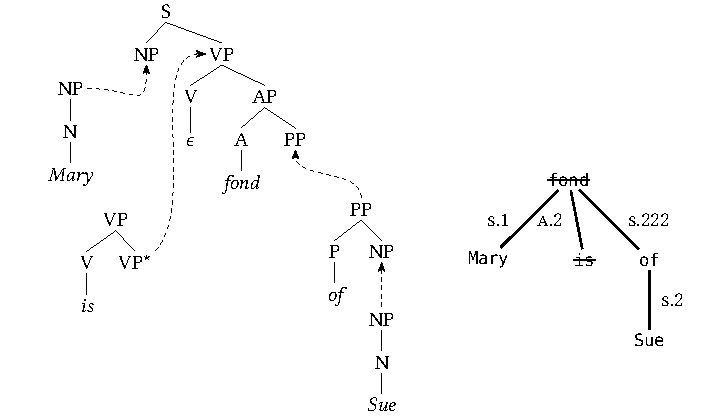
\includegraphics{graphics/abb816.pdf}
\caption{\label{fig-deanchoring-3}Ableitung und Ableitungsbaum für "`Mary \sout{is fond} of Sue"' \citep[Abbildung~4]{Lichte:Kallmeyer:10}}
\end{figure} 
Im Rahmen einer Small-Clause-Analyse adjungiert das finite Verb {\it is} an den Elementarbaum des Prädikats {\it fond}. Dadurch bildet das Finitum nicht mehr den Wurzelknoten des Ableitungsbaums, sondern eine Tochter des Wurzelknotens. Und es kann sogar noch weiter vom Wurzelknoten entfernt sein. \cite{Lichte:Kallmeyer:10} verdeutlichen das anhand der Kontroll\-verb\-kette\is{Kontrolle} in \ref{ex-deanchoring-3}, die durch \cite{Ross:70} bekannt geworden ist:  

\newpage 
\ex. \label{ex-deanchoring-3} I want to try to begin to write a novel, and
\a. Mary \sout{wants to try to begin to write} a play.\label{ex-deanchoring-3-a}
\b. Mary \sout{wants to try to begin} to write a play.\label{ex-ross-70-b}
\c. Mary \sout{wants to try} to begin to write a play.\label{ex-ross-70-c}
\d. Mary \sout{wants} to try to begin to write a play.\label{ex-ross-70-d}
\z. \citep[(2-c)]{Ross:70}
 
Wiederum inspiriert durch die XTAG-Grammatik\is{XTAG} kommen für die LTAG-Model\-lie\-rung von \ref{ex-deanchoring-3} die Elementarbäume in Abbildung~\ref{fig-deanchoring-4} zum Einsatz. Daraus ergibt sich der Ableitungsbaum in Abbildung~\ref{fig-deanchoring-5}, in dem das finite Verb {\it wants} an das maximal übergeordnete Verb der Kontrollverbkette, nämlich {\it to try}, adjungiert. Der Wurzelknoten entspricht jedoch dem maximal untergeordnetem Verb {\it to write}. Das Beispiel zeigt au\ss erdem, dass das finite Verb beliebig tief im \isi{Ableitungsbaum} eingebettet sein kann, da die Kontrollverbkette theoretisch beliebig viele Verben enthalten kann.



Aufgrund der Platzierung des finiten Verbs und des restlichen getilgten Materials in den Ableitungsbäumen der Abbildungen~\ref{fig-deanchoring-3} und~\ref{fig-deanchoring-5} betrachten \cite{Lichte:Kallmeyer:10} den sogenannten \textsc{A-Teilbaum}\is{A-Teilbaum} ("`A-subtree"'), d.\,h.\ den Teilbaum des Ableitungsbaums\is{Ableitungsbaum}, der den Wurzelknoten enthält und deren Kanten Adjunktionen\is{Adjunktion} repräsentieren (also ein {\sc a}-Label haben). Die Annahme ist, dass das finite Verb, wenn es nicht im Wurzelknoten steckt, im \isi{A-Teilbaum} unterhalb des Wurzelknotens zu finden ist. Satzglieder (bzw.\ "`major constituents"'\is{Major Constituent}) bilden auch diejenigen Teilbäume des Ableitungsbaums, deren Wurzelknoten eine sogenannte S-Tochter ist. S-Töchter sind Knoten, die von einem Knoten des A-Teilbaums\is{A-Teilbaum} via einer Substitutionskante\is{Substitution} dominiert werden. Dazu zählen beispielsweise in Abbildung~\ref{fig-deanchoring-5} die Knoten {\tt Mary}, {\tt PRO} und {\tt a\_play}.  Teilbäume mit einer S-Tochter als Wurzelknoten werde ich im Folgenden auch als \textsc{S-Teilbäume}\is{S-Teilbaum} bezeichnen. Die Eingrenzung der Ellipse in Ableitungsbäumen von \cite{Lichte:Kallmeyer:10} kann dann wie in \ref{ex-entankerung-interne-bedingungen} paraphrasiert werden:\footnote{Für die formale Darstellung einer Implementierung der internen Bedingungen verweise ich auf \cite{Lichte:Kallmeyer:10}. Dort wird auch eine Einschränkung erwähnt, um Daten wie \ref{ex-deanchoring-4} auszuschlie\ss en:\\
\fnex{
\ex. \label{ex-deanchoring-4}* \ldots and I want \sout{to} try to begin to write a novel. 

}
Die Einschränkung lautet, dass nur diejenige A-Tochter eines nicht entankerten Knotens entankert werden kann, die die kürzeste \isi{Gorn-Adresse} hat, also am höchsten adjungiert. 
} 
\begin{figure}[p]
\centering
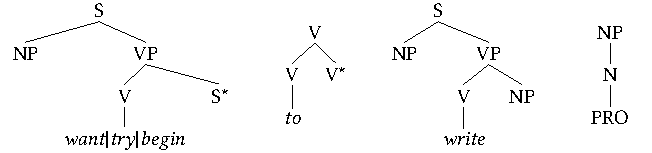
\includegraphics{graphics/abb817.pdf}
\caption{\label{fig-deanchoring-4}Elementarbäume für Kontrollverben im Sinne der XTAG-Grammatik \citep[Abbildung~5]{Lichte:Kallmeyer:10}}
\end{figure}

\begin{figure}[p]
\centering
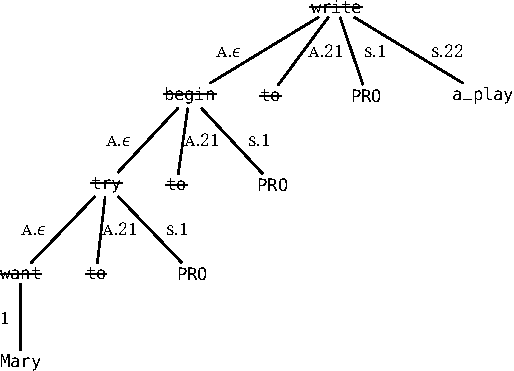
\includegraphics{graphics/abb818.pdf}
\caption{\label{fig-deanchoring-5}Ableitungsbaum für \ref{ex-deanchoring-3-a} \citep[Abbildung~6]{Lichte:Kallmeyer:10}}
\end{figure} 
\clearpage 

\ex. {\bf Interne Bedingungen} (\cite{Lichte:Kallmeyer:10}, informell) \label{ex-entankerung-interne-bedingungen}
\a. Die entankerten Knoten bilden einen verbundenen Teilbaum des Ableitungsbaums.
\b. Falls ein Knoten $v$ des A-Teilbaums entankert wird, dann werden auch alle Knoten im A-Teilbaum entankert, die von $v$ dominiert werden.\label{ex-entankerung-interne-bedingungen-b}
\c. Falls ein Knoten eines S-Teilbaums $\delta$ entankert wird, dann werden auch alle anderen Knoten in $\delta$ entankert.
\e. Mindestens ein Knoten des Ableitungsbaums ist nicht entankert.
%ACHTUNG: Wiederverwendung beim Füllungsansatz!  

Zwar lassen sich damit die zuvor betrachteten Daten erfassen, mit Blick auf andere Gapping-Daten des Englischen erweist sich jedoch diese Eingrenzung (unter einer XTAG-basierten\is{XTAG} Modellierung) \cite{Lichte:Kallmeyer:10} zufolge sowohl als zu permissiv, als auch als zu restriktiv. Zu permissiv ist die Eingrenzung, da sie das Gapping\is{Ellipse!Gapping} mit nur einem Überbleibsel\is{Ellipse!Bare Argument Ellipsis} (oder "`Stripping"') zulässt. Sätze wie \ref{ex-deanchoring-5} werden jedoch traditionell als ungrammatisch beurteilt (siehe z.\,B.\ \citealt[27a]{Jackendoff:71}; \citealt[3]{Johnson:04}):

\ex.  *John gave a book to Mary and Peter \sout{gave a book to Mary}.\\
\citep[(13)]{Lichte:Kallmeyer:10}\label{ex-deanchoring-5}

Zu permissiv ist diese Eingrenzung  au\ss erdem in Fällen, wo Brückenverben\is{Brückenkonstruktion} beteiligt sind. Da  Brückenverben in TAG (und auch in \isi{XTAG}) üblicherweise adjungieren, um weite Abhängigkeiten generieren zu können, und sie dann Teil des A-Teilbaums sind, sollten auch Ellipsen wie in \ref{ex-lk10-17} möglich sein:    

\ex. Larry thinks Sue is nice and \label{ex-lk10-17}
\a. *Sue \sout{thinks} Larry is funny.
\b. *Sue \sout{thinks} Larry \sout{is nice}.
\z. \citep[(17)]{Lichte:Kallmeyer:10}

Leider spricht sich die Literatur gegen die Grammatikalität solcher Daten aus (\citealt[198]{Sag:76}; \citealt[18]{Johnson:04}; \citealt[1149]{Osborne:08}). 

Dagegen ist die Eingrenzung dann zu restriktiv, wenn entgegen der Vorhersage solche Knoten eines A-Teilbaums\is{A-Teilbaum} nicht entankert sind, die darin von einem entankerten Knoten dominiert werden. \cite{Lichte:Kallmeyer:10} geben hierfür die Beispiele in \ref{ex-deanchoring-6}:   

\ex. \label{ex-deanchoring-6}
\a. Mary always finishes her homework, but \\
Peter \sout{finishes}  \sout{his homework} only sometimes. \label{ex-deanchoring-6-a}
\b. Mary is always fond of cheesecake, but \\
Peter \sout{is} only sometimes \sout{fond of cheesecake}. \label{ex-deanchoring-6-b}
\z. \citep[(14),(15)]{Lichte:Kallmeyer:10}

Die Ableitungsbäume dieser Sätze in Abbildung~\ref{fig-deanchoring-6} und \ref{fig-deanchoring-7} zeigen ein unlizenziertes Ent\-ankerungsmuster, da der Knoten {\tt only\_sometimes} nicht entankert ist, obwohl die Eingrenzung in \ref{ex-entankerung-interne-bedingungen-b} das eigentlich vorschreibt. Hier bedarf es also einer Anpassung, die aber in \cite{Lichte:Kallmeyer:10} nicht durchgeführt wird. Dabei liegt eine mögliche Anpassung auf der Hand: Angaben\is{Angabe} werden im \isi{Ableitungsbaum} mit einem speziellen Merkmal versehen und die b-Klausel in \ref{ex-entankerung-interne-bedingungen} so verändert, dass Knoten mit Angabenmarkierung davon ausgenommen werden -- womit auch die a-Klausel obsolet wäre. Da komplexe Knotenlabel unabhängig davon für die Modellierung der externen Bedingungen\is{Entankerung!externe Bedingung}  angenommen werden müssen (siehe unten), ist das kein technischer Sonderweg. Ich möchte diese Anpassungsmöglichkeit hier jedoch nicht weiter ausführen.

\begin{figure}[t]
\centering
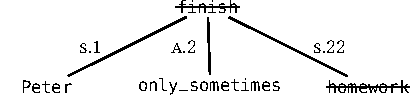
\includegraphics{graphics/abb819.pdf}
\caption{\label{fig-deanchoring-6}Ableitungsbaum für \ref{ex-deanchoring-6-a} \citep[Abbildung~8]{Lichte:Kallmeyer:10}}
\end{figure}

\begin{figure}[t]
\centering
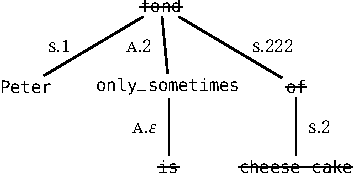
\includegraphics{graphics/abb820.pdf}
\caption{\label{fig-deanchoring-7}Ableitungsbaum für \ref{ex-deanchoring-6-b} \citep[Abbildung~9]{Lichte:Kallmeyer:10}}
\end{figure}
\is{Entankerung!interne Bedingung|)}

\subsection{Vergleich mit \cite{Osborne:08} und \cite{Kobele:09}}

In Abschnitt \ref{sec-tag-ling} wurde bereits erwähnt, dass sich Ableitungsbäume\is{Ableitungsbaum} und Dependenzbäume\is{Dependenzgraph} zwar ähneln, dass aber manche Arten der Komplementation durch unterschiedliche Dominanzverhältnisse repräsentiert werden (siehe Abbildung \ref{fig-TAG-raising2}, S.\,\pageref{fig-TAG-raising2}). Der Ent\-ankerungs\-ansatz ist daher zwar vergleichbar mit dem dependenzstrukturellen Ansatz bei \cite{Osborne:08}, aber es ergeben sich deutliche Unterschiede durch folgenden Umstand: In Dependenzstrukturen\is{Dependenzgraph} ist das finite Verb, zumindest bei komplementiererfreien Hauptsätzen, leicht zu identifizieren, denn es bildet bei Osborne immer den \isi{Wurzelknoten} des Dependenzgraphen. Bei Ableitungsbäumen ist dies dagegen nicht so. Ist das Finitum nämlich der lexikalische Anker eines Hilfsbaums\is{Hilfsbaum}, was etwa bei Hilfs-\is{Hilfsverb}, Anhebungs-\is{Anhebung} und Kontrollverben\is{Kontrolle} aber auch bei Kopulakonstruktionen\is{Kopulakonstruktion} zutrifft, dann entspricht es eben nicht dem Wurzelknoten des TAG"=Ableitungsbaums. Man beachte, dass diese Eigenschaft auch eine Folge des Valenzprinzips\is{Wohlgeformtheitsprinzip!Valenzprinzip für TAG} für LTAG ist (siehe S.\,\pageref{ex-valenzprinzip-tag}).  

Augenfällig wird dieser Unterschied beispielsweise, wenn man den Ableitungsbaum in Abbildung~\ref{fig-deanchoring-5} und den entsprechenden Dependenzbaum\is{Dependenzgraph}, der in Abbildung~\ref{fig-deanchroing-8} dargestellt wird (vgl.\ \citealt[(110)]{Osborne:08}), gegenüberstellt.
\begin{figure}[t]
\centering
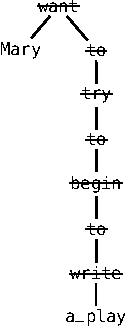
\includegraphics{graphics/abb821.pdf}
\caption{\label{fig-deanchroing-8}Dependenzgraph für \ref{ex-deanchoring-3-a} aus \citet[(110)]{Osborne:08}}
\end{figure}
Der Dependenzbaum\is{Dependenzgraph} kehrt bestimmte Dominanzverhältnisse des Ableitungsbaums um: Die Verben dominieren einander entsprechend ihrer Rangordnung und auch der Statusmarkierer {\it to} dominiert das jeweils statusmarkierte Verb. Eine interessante Frage ist nun, ob in einem solchen Dependenzbaum nicht nur die Identifizierung des finiten Verbs leichter fällt, sondern auch die Identifizierung potentieller Überbleibsel. Doch letzteres scheint nicht der Fall zu sein, wenn man Osbornes Ausführungen zum Ma\ss stab nimmt. Da seine Dependenzstrukturen\is{Dependenzgraph} keinerlei syntaktische Annotation aufweisen, muss er bei der Definition eines potentiellen Überbleibsels (oder "`major constituent"'\is{Major Constituent}, \citealt[1146]{Osborne:08}) auf den vagen Begriff der Prädikatkette ("`predicate chain"') zurückgreifen. Ein Ableitungsbaum bietet hier per se mehr Anhaltspunkte für eine Charakterisierung, z.\,B.\ die Unterscheidung zwischen Substitutionskanten und Adjunktionskanten, die eine Charakterisierung mittels A-Teilbäume\is{A-Teilbaum} möglich macht.

Nur schwer zu vergleichen ist der Entankerungsansatz mit dem MG-Ansatz\is{Minimalist Grammar} von \cite{Kobele:09}. Zwar ist beiden Ansätzen der Bezug auf Ableitungsstrukturen gemein, doch die jeweiligen Ableitungsstrukturen unterliegen ganz verschiedenen Repräsentationsfunktionen. Die Innenknoten eines MG-Ableitungsbaums repräsentieren bei Kobele nämlich Merge- und Move-Operationen, während dessen Blätter durch lexikale Elementarstrukturen besetzt werden. Dadurch und durch das Fehlen einer erweiterten Lokalitätsdomäne\is{erweiterte Lokalitätsdomäne} im MG-Formalismus ist die Prädikat-Argument-Struktur im Ableitungsbaum nicht sichtbar. Das scheint für die Erfassung von VP-Ellipsen\is{Ellipse!VP-} im Englischen, denen sich Kobele widmet, kein Nachteil zu sein. Ob sich sein MG-Ansatz ohne Weiteres auf Gapping-Daten\is{Ellipse!Gapping} übertragen lässt, scheint mir aber fraglich.

\subsection{Externe Bedingungen}\label{sec-deanchoring-extern}\is{Entankerung!externe Bedingung|(}

Die Entankerung muss auch durch eine gewisse Ähnlichkeit zwischen Ellipse und Antezedens lizenziert sein, die in den sogenannten externe Bedingungen festgehalten wird. Die externen Bedingungen operieren wie die internen Bedingungen auf Ableitungsbäumen, betrachten aber immer Paare verschiedener Ableitungsbäume, nämlich zum einen den Ableitungsbaum mit der Entankerung und zum anderen den \isi{Ableitungsbaum} mit deren \isi{Antezedens}.\footnote{In einer Koordinationsellipse\is{Ellipse!Koordinations-} betrachten wir also diejenigen Teilbäume des Ableitungsbaums, die den Konjunkten der Koordination entsprechen, und in einer Adjazenzellipse\is{Ellipse!Adjazenz-} die Ableitungsbäume aufeinander folgender Sätze. Bei einer freien Ellipse\is{Ellipse!ohne Antezedens} steht kein overter Ableitungsbaum zur Verfügung. Dort müsste die Diskursstruktur etwas entsprechendes beisteuern.} Die formale Explikation der externen Bedingungen, die \cite{Lichte:Kallmeyer:10} angeben, lässt sich folgenderma\ss en paraphrasieren:

\ex. {\bf Externe Bedingungen} (\citealt{Lichte:Kallmeyer:10}, informell) \label{ex-entankerung-externe-bedingungen}
\a. Jeder entankerte Knoten hat genau einen Antezedensknoten.
\b. Ein entankerter Knoten und sein Antezedensknoten nehmen dieselbe Position im jeweiligen Ableitungsbaum ein, d.\,h.\ die Konkatenation der Kantenlabel entlang des Dominanzpfads ist identisch. (Pfadidentität)
\c. Ein entankerter Knoten und sein Antezedensknoten haben ein partiell identisches Knotenlabel. (partielle Labelidenität)    

\newpage
Man beachte, dass diese externen Bedingungen keinen Isomorphismus, sondern nur einen Homomorphismus zwischen Ellipse und Antezedens bewirken, da nur sichergestellt wird, dass jeder entankerte Knoten auf einen Antezdensknoten abgebildet wird, nicht jedoch, dass auch jeder Antezdensknoten auf einen entankerten Knoten abgebildet wird. Ellipsen können demnach kleiner sein als ihre Antezedenten. Dies ist aber insofern konsequent, als ja die internen und externen Bedingungen die Frage beantworten sollen, welche Knoten entankert werden können, und  nicht, was der korrekte Rekonstruktionsumfang einer Ellipse ist.\footnote{Um den korrekten Rekonstruktionsumfang einer Ellipse zu erhalten, müsste man zuerst einmal festlegen, welchen Umfang ein \isi{Antezedens} in einem Ableitungsbaum überhaupt haben kann. Im vorliegenden Fall könnte man dafür analog zu den internen Bedingungen aus \ref{ex-entankerung-interne-bedingungen} die folgenden Antezdensbedingungen formulieren:\\
\fnex{
\ex. {\bf Antezedensbedingungen} \label{ex-entankerung-antezedensbedingungen}
\a. Die Antezdensknoten bilden einen Teilbaum des Ableitungsbaums.
\b. Falls ein Knoten $v$ des A-Teilbaums ein Antezedensknoten ist, dann sind auch alle Knoten im A-Teilbaum ein Antezdensknoten, die von $v$ dominiert werden.
\c. Falls ein Knoten eines S-Teilbaums $\delta$ ein Antezedensknoten ist, dann sind auch alle anderen Knoten in $\delta$ Antezedensknoten.

}
Schlie\ss lich müsste noch die a-Klausel der externen Bedingungen in \ref{ex-entankerung-externe-bedingungen} angepasst werden: Jeder entankerte Knoten hat genau einen Antezedensknoten und jeder Antezedensknoten hat genau einen entankerten Knoten.} 

\cite{Lichte:Kallmeyer:10} zufolge erweist es sich als zu strikt, die vollständige Identität der Label der betroffenen Knoten zu fordern. Bestimmte Möglichkeiten der morphosyntaktischen Divergenz zwischen Ellipse und Antezedens werden damit übergangen, wie z.\,B.\ die Numerus-Divergenz\is{Numerus} der Verben in \ref{ex-deanchoring-7}:  

\ex. \label{ex-deanchoring-7} I am flying to Europe, and you \sout{are flying} to Asia. \hfill \citep[(4)]{Osborne:08}

Auch wenn nicht vorgegeben ist, welches Label die Elementarbäume der Hilfsverben\is{Hilfsverb} {\it am} und {\it are} in einer konkreten Implementierung erhalten, so erhalten sie in jedem Fall unterschiedliche Knotenlabel. Nur so kann die Bijektivität zwischen Ableitungsbäumen und abgeleiteten Bäumen bewahrt werden. 
\cite{Lichte:Kallmeyer:10} schlagen daher eine Ausdifferenzierung der Knotenlabel vor, indem die Knoten im Ableitungsbaum statt eines atomaren Labels Merkmalsstrukturen\is{Merkmalsstruktur} wie in Abbildung~\ref{fig-deanchoring-9} tragen. 
\begin{figure}[t]
\centering
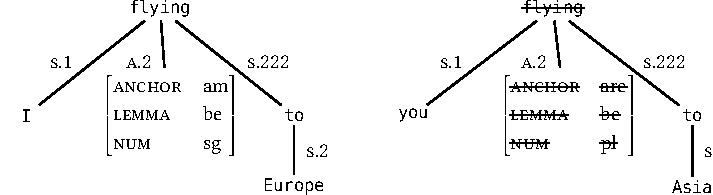
\includegraphics{graphics/abb822.pdf}
\caption{\label{fig-deanchoring-9}Ableitungsbäume mit komplexen Knotenlabel für die Modellierung morphosyntaktischer Divergenzen zwischen Ellipse und Antezedens \citep[(7)]{Lichte:Kallmeyer:10}}
\end{figure}
Mittels dieser Merkmalsstrukturen\is{Merkmalsstruktur} kann die Knotenlabelidentität auf bestimmte Merkmale, z.\,B.\ {\sc lemma}, beschränkt werden, ohne das {\sc num(erus)}-Merkmal\is{Numerus} einzubeziehen. Die Trennung von zulässigen und unzulässigen Divergenzen lässt sich so recht einfach modellieren. Zu den unzulässigen Divergenzen zählen \cite{Lichte:Kallmeyer:10} au\ss erdem noch das \isi{Genus Verbi} und die Tempusmorphologie\is{Tempus}. Möglicherweise zählt auch die Satzstellung (Topikalisierung vs.\ Basisstellung) dazu. Der Tatsache, dass phonetisch sichtbare Divergenzen nur bei Verben auf"|treten können, nicht aber bei Nominalphrasen (siehe \ref{ex-koord-25} auf S.\,\pageref{ex-koord-25}), kann man damit ebenfalls ohne Weiteres gerecht werden.

Ein interessanter Aspekt dieser komplexen Knotenlabel, den \cite{Lichte:Kallmeyer:10} nicht erwähnen, besteht darin, dass mit ihrer Hilfe das finite Verb im Ableitungsbaum markiert werden kann. Damit wäre es bei der Entankerung im Rahmen der internen Bedingungen\is{Entankerung!interne Bedingung} leichter identifizierbar, insbesondere wenn es nicht dem Wurzelknoten entspricht. Ich werde gleich bei der Anpassung der Entankerung für das TT-MCTAG-Modell des Deutschen darauf zurückgreifen.

Anders als die Label von Ellipseknoten und Antezedensknoten scheinen deren Pfade im jeweiligen Ableitungsbäumen immer identisch zu sein. Als Beleg führen \cite{Lichte:Kallmeyer:10} den ungrammatischen Satz \ref{ex-deanchoring-path} an, in dem das eingebettete Verb {\it ordered} als Antezedens einer Ellipse dienen soll:  

\ex. *Since Peter ordered a beer, the waitress instantly reached for the fridge and Mary \sout{ordered} a whole chicken. \hfill \citep[(10)]{Lichte:Kallmeyer:10}\label{ex-deanchoring-path}

Da sich im \isi{Ableitungsbaum} für \ref{ex-deanchoring-path} die Pfade von Ellipseknoten und Antezedensknoten in der Länge  unterscheiden müssen, ist \ref{ex-deanchoring-path} nicht derivierbar. Aber auch in subtileren Fällen, wo Ellipse und Antezedens unmittelbare Satzglieder der Konjunktsätze bilden, macht die Bedingung der Pfadidentität interessante Vorhersagen. Beispielsweise verhindert sie auch Ellipse der in \ref{ex-deanchoring-path-2} angedeuteten Art, deren grammatikalischer Status mir allerdings unklar ist:

\ex. \label{ex-deanchoring-path-2} 
?Peter will first meet Susi and later this afternoon John \sout{will meet} Mary.
%?*Mary always finishes her homework, but \\ only sometimes Peter \sout{finishes}  \sout{his homework}. 

Das Eigentümliche dieser \isi{Koordination} ist die divergierende Stellung der temporalen Bestimmungen {\it first} und {\it later this afternoon}: Während im ersten Konjunkt {\it first} präverbal zwischen dem Hilfsverb und dem Vollverb steht, befindet sich im zweiten Konjunkt {\it later this afternoon} in einer satzinitialen Position. Da in der XTAG-Grammatik\is{XTAG} satzinitiale Adverbien\is{Angabe} am Wurzelknoten des Elementarbaums des Vollverbs adjungieren, unmittelbar präverbale Adverbien aber am tieferliegenden VP-Knoten, ergibt sich eine Pfaddivergenz zwischen den Ableitungsbäume wie in Abbildung~\ref{fig-deanchoring-path} dargestellt. 
\begin{figure}[t]
\centering
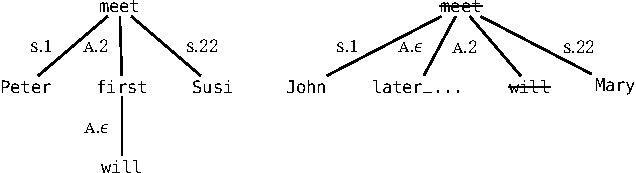
\includegraphics{graphics/abb823.pdf}
\caption{\label{fig-deanchoring-path}Ableitungsbäume der Konjunkte in \ref{ex-deanchoring-path-2}}
\end{figure}
Die Pfaddivergenz zwischen dem Antezedensknoten und dem Ellipseknoten von {\tt will} ist hier entscheidend und verhindert  die Derivation von \ref{ex-deanchoring-path-2}. Man beachte jedoch, dass bereits leichte Veränderungen an \ref{ex-deanchoring-path-2} diese Pfaddivergenz verschwinden lassen: die postverbale Positionierung von {\it later this afternoon} (vgl.\ \ref{ex-deanchoring-path-3-a}), das dann an VP adjungieren kann, oder die Herausnahme des Hilfsverbs\is{Hilfsverb} (vgl.\ \ref{ex-deanchoring-path-3-b}): 

\ex.
\a. ?Peter will first meet Susi and then John \sout{will meet} Mary later this afternoon.\label{ex-deanchoring-path-3-a}
\b. ?Peter first met Susi and later this afternoon John \sout{met} Mary.\label{ex-deanchoring-path-3-b} 

Man kann sicherlich darüber streiten, ob \ref{ex-deanchoring-path-3-b} wirklich wesentlich besser ist als die ausgefilterte Variante in \ref{ex-deanchoring-path-2}.
\is{Entankerung!externe Bedingung|)}   


\section{Füllung} \label{sec-fuellung}\is{Füllung|(}

Den Füllungsansätzen im Rahmen des TAG-Frameworks ist gemein, dass Null-Anaphern\is{Null-Anapher} anhand von Form von Elementarbäumen mit phonetisch leerem Anker implementiert werden, die auch "`ghost trees"' \citep{Seddah:Sagot:06} oder Dummy"=Elementarbäume genannt werden. Beispiele für einen nominalen und einen verbalen \isi{Dummy-Elementarbaum} sind in Abbildung~\ref{fig-tag-fuellung-1} dargestellt.
\begin{figure}[t]
\centering
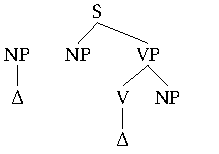
\includegraphics[angle=90]{graphics/abb824.pdf}
\caption{\label{fig-tag-fuellung-1}Ein nominaler und ein verbaler Dummy-Elementarbaum im Füllungsansatz}
\end{figure}  
Im Unterschied zum Verschmelzungsansatz\is{Verschmelzung} knüpfen die Füllungsansätze einen Dummy"=Elementarbaum nicht direkt an ein overtes Antezedens, etwa durch die Bündelung in einer Baummenge. Die Lizenzierung der Dummy-Elementarbäume erfolgt stattdessen entweder durch Merkmalsspezifikationen in dessen Knotenlabel, oder durch Bedingungen auf dem Ableitungsbaum. Man kann hier wie bei der Entankerung von den internen Bedingungen sprechen. Der Bezug zwischen Ellipse und Antezedens, oben als externe Bedingungen verhandelt, wird ebenfalls indirekt hergestellt, beispielsweise über den Ableitungsbaum oder die semantische Form.

Neben diesen Gemeinsamkeiten von TAG-Füllungsansätzen gibt es zwischen ihnen wesentliche Unterschiede abhängig davon, welches Füllungsparadigma jeweils umgesetzt wird: Entweder sind Füllungen strukturiert, d.\,h.\ es besteht eine phrasenstrukturelle Isomorphie zwischen Ellipse und Antezedens (im Sinne der Empty Structures Hypothesis), oder Füllungen sind unstrukturiert, d.\,h.\ es besteht dieser Isomorphismus nicht (im Sinne der Non-Expansion Hypothesis).
\is{Füllung|)}  



\subsection{\cite{Seddah:Sagot:06}}
\largerpage
Die einzige bisher veröffentlichte Arbeit, die im Rahmen des TAG-Frameworks die Füllungsstrategie verfolgt, ist meines Wissens \cite{Seddah:Sagot:06}. Djam\'e Seddah und Beno\^{i}t Sagot übertragen hier eine Methode auf die Ellipsenmodellierung, die zur Modellierung von Kontrollkonstruktionen in \cite{Seddah:Gaiffe:05} entwickelt worden ist. In diesen Arbeiten werden die Dummy"=Elementarbäume\is{Dummy-Elementarbaum}, oder "`ghost trees"', über den \isi{Ableitungsbaum} sowohl lizenziert als auch rekonstruiert. Der Ableitungsbaum wird dabei als Menge von Chart-Objekten ("`derivation item"') repräsentiert, wie sie beim deduktiven Parsing \citep{Shieber:etal:95} gebräuchlich sind. \cite{Seddah:Sagot:06} beschränken sich auf die Angabe von zwei deduktiven Regeln auf diesen Chart-Objekten, je eine für verbale und nominale Dummy-Elementarbäume. Was sie strukturell implizieren und wie sie die Rekonstruktion der Dummy-Elementarbäume bestimmen, ist in Abbildung~\ref{fig-tag-fuellung-2} zusammengefasst und soll hier nur informell wiedergegeben werden:
\begin{enumerate}
  \item (Gapping) Ein verbaler Dummy-Elementarbaum $\delta_v$ kann den \isi{Wurzelknoten} desjenigen Teilbaums des Ableitungsbaums bilden, der dem zweiten Konjunkt entspricht.
  \item (Argument"|tilgung) Ein nominaler Dummy-Elementarbaum $\delta_n$ kann die Tochter des Wurzelknotens $\alpha_2$ desjenigen Teilbaums bilden, der dem zweiten Konjunkt entspricht, sofern $\alpha_2$ kein Dummy-Elementarbaum ist.    
\end{enumerate}
\begin{figure}[t]
\centering
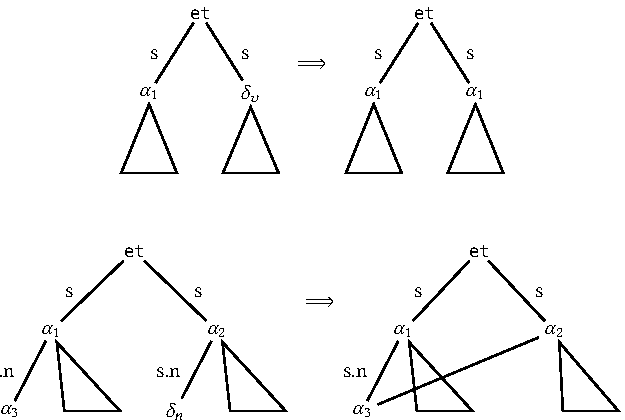
\includegraphics{graphics/abb825.pdf}
\caption{\label{fig-tag-fuellung-2}Lizenzierung und Rekonstruktion der Dummy"=Elementarbäume im Ableitungsbaum gemä\ss\ \cite{Seddah:Sagot:06}}
\end{figure} 
Diese beiden Regeln erfassen nur einfache Fälle von Gapping und Argument"|tilgung. Die Position der getilgten (oder vielmehr $\delta$-gefüllten) Argumente ist zudem vollkommen unbeschränkt und die Regeln daher übergenerierend. Seddah und Sagot begnügen sich offensichtlich mit einer groben Skizzierung des Verfahrens, die aber ausreicht, um die \isi{Rekonstruktion} von Dummy"=Elementarbäumen anhand des Ableitungsbaums zu demonstrieren. Die Rekonstruktion besteht im Grunde darin, die Instanzen der Dummy-Elementarbäume aus dem Ableitungsbaum zu entfernen, so dass sich die Ableitungsstruktur der vermeintlichen semantischen Dependenzstruktur\is{Dependenzgraph} annähert:\newpage
\begin{enumerate}
  \item (Gapping) Im Ableitungsbaum erhält der Knoten eines verbalen Dummy"=Elementarbaums $\delta_v$ das Label des Antezedens $\alpha_1$. Der Antezedenselementarbaum wird quasi kopiert.
  \item (Argument"|tilgung) Im Ableitungsbaum wird der Knoten eines nominalen Dummy"=Elementarbaums $\delta_n$ mit dem Knoten des Antezedensbaums $\alpha_3$ fusioniert. Der resultierende Knoten trägt weiterhin das Label $\alpha_3$ und wird von $\alpha_1$ und $\alpha_2$ geteilt.
\end{enumerate}
Die Fusion von Knoten im Ableitungsbaum kennen wir bereits aus dem Verschmelzungsansatz\is{Verschmelzung} von MCTAG-LSD (vgl.\ Abbildung~\ref{fig-seddah-rnr-2}). Dort wird jedoch die Fusion durch lexikalische Spezifikationen, den sogenannten Sharing-Links, reglementiert, wohingegen \cite{Seddah:Sagot:06} die Fusion allein anhand von Eigenschaften des Ableitungsbaums einschränken. Die Kopieroperation für die \isi{Rekonstruktion} verbaler Dummy-Elementarbäume\is{Dummy-Elementarbaum} fehlt bei MCTAG-LSD und wird durch eine Antezedens-Ellipse-Bündelung qua Baummenge ersetzt. \cite{Seddah:08} begründet diesen Schritt mit dem Verweis auf die Ellipse-Antezedens-Divergenzen in \ref{ex-fuellung-1}: 

\ex. \label{ex-fuellung-1}
\a. Napoleon prit du poids et \sout{prit} beaucoup de pays. \label{ex-fuellung-1-a}
\b. Jean est un r\'epublicain et \sout{Jean est} fier de l'\^{e}tre. \label{ex-fuellung-1-b} 
\z. \citep[Abbildung~1]{Seddah:08}

Die Divergenz in \ref{ex-fuellung-1-a}, eine sogenannte \isi{Zeugma-Konstruktion}, besteht auf der Ebene der lexikalischen Semantik, wohingegen die Divergenz in \ref{ex-fuellung-1-b} die Valenzstruktur des Kopulaverbs\is{Kopulakonstruktion} {\it est} betrifft. Die Modellierung solcher und anderer Ellipse-Antezedens-Divergenzen lässt sich wohl nicht mit einer Kopieroperation auf atomaren Knotenlabels bewerkstelligen. Wie aber bei der Entankerung gezeigt wurde (vgl.\ Abbildung~\ref{fig-deanchoring-9}, S.\,\pageref{fig-deanchoring-9}), kann man mittels komplexer Knotenlabels diejenigen Eigenschaften eines Elementarbaums unterscheiden, die für die notwendige Parallelität von Ellipse und Antezedens relevant sind. Möglicherweise lässt sich diese Methode auf den Füllungsansatz von \cite{Seddah:Sagot:06} übertragen.

Bei den Fällen von Gapping\is{Ellipse!Gapping} mit nicht-komplexem Antezedens, die \cite{Seddah:Sagot:06} betrachten, spielt die Unterscheidung zwischen strukturierten und unstrukturierten Füllungen naturgemä\ss\ noch keine Rolle. Im Folgenden werde ich auf Gappingdaten mit komplexen Antezedens eingehen, dabei aber nicht den Ansatz in \cite{Seddah:Sagot:06} weiterführen, sondern den Vergleich mit dem Entankerungsansatz von \cite{Lichte:Kallmeyer:10} suchen.
 

\subsection{Strukturierte Füllungen}\is{Füllung!strukturierte|(}  

Entsprechend Wasows ESH\is{Empty Structures Hypothesis (ESH)} können strukturierte Füllungen aus komplexen Phrasenstrukturen mit mehreren opaken Dummy-Terminalen ($\Delta$) bestehen. Oben in \ref{ex-fuellung-2-c} gab ich folgendes Beispiel:

\ex. I want to try to begin to write a novel, and Mary [$\Delta$ [$\Delta$ [$\Delta$ [$\Delta$  a play]]]].\label{ex-fuellung-2-c-wdh}  

%da strukturierte Füllungen eine phrasenstrukturelle Isomorphie zum Antezedens aufweisen sollen (entsprechend Wasows ESH),
Es wurde schon angemerkt, dass eine gewisse strukturelle Übereinstimmung mit der PF-Til\-gung\is{PF-Tilgung} besteht \citep[6]{Winkler:Schwabe:03} und auch mit der \isi{Entankerung}. Der Entankerungsansatz verwendet ja zur Ellipsenmodellierung ebenfalls Phrasenstrukturen mit Dummy"=Terminalen -- allerdings als Folge einer Nachbearbeitung, d.\,h.\ ohne lexikalischen Status. Es verwundert also nicht, dass die internen Bedingungen\is{Entankerung!interne Bedingung} aus \cite{Lichte:Kallmeyer:10}, die in \ref{ex-entankerung-interne-bedingungen} festgehalten wurden und für das Englische gelten, beinahe direkt in den Füllungsansatz übernommen werden können. Dafür bedarf es im Wesentlichen nur einer Ersetzung von Ausdrücken der Art "`entankert werden"' durch Ausdrücke der Art "`Dummy-Elementarbäume sein"':\is{Füllung!interne Bedingung}\is{Dummy-Elementarbaum}\is{Ableitungsbaum}     

\ex. {\bf Interne Bedingungen für die Verwendung der Dummy"=Elementarbäume} (Strukturierte Füllungen) \label{ex-fuellung-interne-bedingungen-1}
\a. Die Knoten für die Dummy"=Elementarbäume bilden einen Teilbaum des Ableitungsbaums.
\b. Falls ein Knoten $v$ des A-Teilbaums\is{A-Teilbaum} ein Dummy-Elementarbaum ist, dann sind auch alle Knoten im A-Teilbaum Dummy"=Elementarbäume, die von $v$ dominiert werden.
\c. Falls ein Knoten eines S-Teilbaums\is{S-Teilbaum} $\delta$ ein Dummy-Elementarbaum ist, dann sind auch alle anderen Knoten in $\delta$ Dummy"=Elementarbäume.
\e. Mindestens ein Knoten des Ableitungsbaums ist kein Dummy"=Elementarbaum.

\begin{sloppypar} Für die \isi{Rekonstruktion} strukturierter Füllungen bietet sich wieder der Weg über den Ableitungsbaum an und die Adaption der externen Bedingungen aus dem Entankerungsansatz\is{Entankerung!externe Bedingung} (siehe S.\,\pageref{sec-deanchoring-extern}). Der Homomorphismus zwischen Ellipse und Antezedens drückt sich dann darin aus, dass im Ellipse-Ableitungsbaum jeder Knoten eines Dummy-Elementarbaums\is{Dummy-Elementarbaum} auf einen pfadidentischen und partiell labelidentischen Knoten des Antezedens-Ableitungsbaums abgebildet werden kann.\end{sloppypar}   

\newpage
Die enge Kopplung an den Ableitungsbaum des Antezdens dämmt zugleich eine Gefahr ein, die im lexikalischen Status der Dummy-Elementarbäume\is{Dummy-Elementarbaum} lauert. Für die Generierung strukturierter Füllungen wie in \ref{ex-fuellung-2-c-wdh} benötigt man nämlich Dummy-Elementarbäume, die rekursiv aneinander adjungieren können. Damit ist es jedoch möglich, für einen beliebigen Satz mit Gapping\is{Ellipse!Gapping} unendlich viele syntaktische Derivationen durchzuführen. Der Kontext in Form eines Antezdens-Ableitungsbaums hilft eine solche derivationelle Explosion zu verhindern, indem z.\,B.\ maximal so viele Dummy-Elementarbauminstanzen in der Derivation der Ellipse erlaubt sind, wie Elementarbauminstanzen in der Derivation des Antezedenssatzes verwendet werden. Dummy-Elementarbäume wären demnach trotz ihres lexikalischen Status keine gewöhnlichen Elementarbäume, denn ihre Instanziierung wird satzextern restringiert.
\is{Füllung!strukturierte|)}

\subsection{Unstrukturierte Füllungen}\is{Füllung!unstrukturierte|(}

Wenn keine phrasenstrukturelle Isomorphie zwischen Ellipse und Antezedens verlangt wird,\footnote{Dies ist möglicherweise weniger strikt als die von Wasow formulierte NEH\is{Non-Expansion Hypothesis (NEH)} (siehe Abschnitt~\ref{sec-ellipsenanalyse-wege}), die nur atomare Füllungen vorzusehen scheint.} kann statt der strukturierten Füllung in \ref{ex-fuellung-2-c-wdh} auch die unstrukturierte Füllung in \ref{ex-fuellung-3-c}, hier wiederholt als \ref{ex-fuellung-3-c-wdh}, eingesetzt werden:
  
\ex. I want to try to begin to write a novel, and Mary $\Delta$ a play.\label{ex-fuellung-3-c-wdh}
  
Da hierfür auf rekursiv adjungierende Dummy-Elementarbäume\is{Dummy-Elementarbaum} verzichtet werden kann, lassen sich die internen Bedingungen für unstrukturierte Füllungen kürzer fassen als die in \ref{ex-fuellung-interne-bedingungen-1}. Der \isi{A-Teilbaum} und die S-Teilbäume\is{S-Teilbaum} des Ableitungsbaums\is{Ableitungsbaum} enthalten dann nämlich maximal einen Knoten mit Dummy"=Elementarbauminstanz:\is{Füllung!interne Bedingung}

\ex. {\bf Interne Bedingungen für die Verwendung der Dummy"=Elementarbäume} (Unstrukturierte Füllungen) \label{ex-fuellung-interne-bedingungen-2}
\a. Falls ein Knoten $v$ des A-Teilbaums ein Dummy-Elementarbaum ist, dann ist $v$ entweder der \isi{Wurzelknoten} oder ein \isi{Blatt} des A"=Teilbaums.
\b. Falls ein Knoten $v$ eines S-Teilbaums $\delta$ ein Dummy-Elementarbaum ist, dann ist $v$ der einzige Knoten in $\delta$.
\c. Mindestens ein Knoten des Ableitungsbaums ist kein Dummy"=Elementarbaum.
 
Die unstrukturierte Füllung mit Dummy-Elementarbäumen ist also, was die Syntax betrifft, weniger aufwändig als die strukturierte Füllung\is{Füllung!strukturierte} bzw.\ \isi{Entankerung}, da keine vollständige Derivation der Ellipse durchgeführt wird und der Ableitungsbaum kleiner ausfällt. Zudem ist der Gefahr einer derivationellen Explosion, von der ich oben im Zusammenhang mit strukturierten Füllungen sprach, die Grundlage entzogen, womit auch auf eine spezielle kontextuelle Restringierung der Dummy-Elementarbaumverwendung verzichtet werden kann.

Der geringere Aufwand in der Syntax wird jedoch mit einem erhöhten Aufwand in der \isi{Rekonstruktion} der Füllungen, d.\,h.\ in den externen Bedingungen\is{Füllung!externe Bedingung}, erkauft. Bei unstrukturierten Füllungen wie in \ref{ex-fuellung-3-c-wdh}, die ein komplexes \isi{Antezedens} besitzen, muss die Rekonstruktion qua \isi{Ableitungsbaum} neue Wege gehen, da eine bijektive Korrelierung von Knoten nicht möglich ist: Der Knoten eines Dummy-Elementarbaums\is{Dummy-Elementarbaum} $\delta$ steht nun einer Menge von Knoten $V_{\mathit{Ant}}$ im Ableitungsbaum des Antezedenssatzes $D_{\mathit{Ant}}$ gegenüber. Was lässt sich über $V_{\mathit{Ant}}$ sagen? Sofern man die XTAG-Analyse\is{XTAG} der Antezedenssätze zugrunde legt, bildet $V_{\mathit{Ant}}$ einen Teilbaum von $D_{\mathit{Ant}}$, der auch den Wurzelknoten von $D_{\mathit{Ant}}$ umfasst. Beim Gapping in \ref{ex-fuellung-3-c-wdh} kann man zudem erkennen, dass die Kanten zwischen Knoten aus $V_{\mathit{Ant}}$ Adjunktionen repräsentieren. Es begegnet uns also hier wieder der Begriff des A-Teilbaums\is{A-Teilbaum}, der im Rahmen des Entankerungsansatzes zur Charakterisierung der Ellipse und ihrer Überbleibsel verwendet wurde. 

Die \isi{Rekonstruktion} unstrukturierter Füllungen kann aber auch mittels der (Diskurs-)Seman\-tik erfolgen, was u.\,a.\ \cite{Dalrymple:etal:91}  vorschlagen.\footnote{Siehe \citet[68f]{Hardt:93} für kritische Anmerkungen und einen alternativen Vorschlag und \cite{Winkler:Schwabe:03} für Referenzen neueren Datums.} Grob gesagt besteht deren Ansatz darin, die Bedeutung einer Füllung ad hoc durch Unifikation höherer Ordnung ("`higher-order unification"') bzw.\ durch prädikatenlogische Gleichungen aus dem Antezedenssatz zu gewinnen, beispielsweise den $\lambda$-Term in \ref{ex-fuellung-4} für den Gappingfall in \ref{ex-fuellung-3-c-wdh}:

\ex. \label{ex-fuellung-4}$\lambda x \, \lambda y. ${\tt want($x$,try(begin(write($y$))))}   

\largerpage
Dieser $\lambda$-Term kann daraufhin mit den Bedeutungen der Überbleibsel kombiniert werden. Der Gleichungsansatz besticht also durch ein hohes Ma\ss\ an Flexibilität, das insbesondere bei der Modellierung strikter und nicht-strikter ("`sloppy"') Referenzidentität nötig ist. Diese Arbeit klammert diesen vieldiskutierten Aspekt der Semantik von Ellipsen jedoch wohlweislich aus. Ausklammern möchte ich auch den in \cite{Babko-Malaya:06} skizzierten LTAG-Ansatz, der die semantische \isi{Rekonstruktion} mittels einer unterspezifizierten LTAG-Semantik modelliert. Darauf ausführlich einzugehen, würde den thematischen Rahmen dieser Arbeit sprengen.
\is{Füllung!unstrukturierte|)}

\subsection{Lizenzierung über den abgeleiteten Baum}

Die Verwendung der Dummy-Elementarbäume\is{Dummy-Elementarbaum} kann alternativ durch den abgeleiteten Baum\is{abgeleiteter Baum} geregelt werden, d.\,h.\ durch den Einsatz geeigneter Merkmale in den Knotenlabeln der Elementarbäume und durch deren Unifikation bei Substitution und Adjunktion. Diese Methode ist ausdrucksstark genug für die Implementierung der internen Bedingungen\is{Füllung!interne Bedingung} in \ref{ex-fuellung-interne-bedingungen-1} und \ref{ex-fuellung-interne-bedingungen-2}, da die dort zugelassenen Dominanzpfade im Ableitungsbaum durch reguläre Ausdrücke beschrieben werden können. 
Man scheint also die Wahl zu haben zwischen Ableitungsbäumen und abgeleiteten Bäumen als Grundlage für die Lizenzierung der Dummy-Elementarbäume. Darin liegt ein wesentlicher Unterschied zum Entankerungsansatz: Die Lizenzierung der \isi{Entankerung} auf Grundlage des abgeleiteten Baums ist im vorgestellten Entankerungsansatz schwieriger, da dort zunächst gewöhnliche Elementarbäume verwendet und erst postderivationell entankert werden.

Von solchen Implementierungsdetails abgesehen, die auch mit der Einnahme einer Sprachgenerierungsperspektive bzw.\ Sprachverarbeitungsperspektive zusammenhängen, verhalten sich Entankerung und (strukturierte) Füllung bei der Formulierung der internen und externen Bedingungen deswegen sehr ähnlich, weil in beiden Fällen der Ableitungsbaum als Bezugsgrö\ss e genutzt werden kann. Wenn ich also im nächsten Abschnitt eine Übertragung auf das TT-MCTAG-Modell und das Deutsche vornehme, dann ist die Wahl zwischen Entankerung und Füllungen zunächst einmal nebensächlich.     



\section{Entankerung/Füllung mit TT-MCTAG}\label{sec-deanchoring-ttmctag}

Der Anschauungsschwerpunkt bei der Vorstellung des Entankerungsansatzes in \cite{Lichte:Kallmeyer:10} lag auf einem LTAG-Fragment des Englischen. In diesem Abschnitt möchte ich stattdessen das TT-MCTAG-Modell aus Kapitel~\ref{sec-ttmctag} und die Gappingregeln\is{Gappingregel} aus Kapitel~\ref{chap-ellipse} in den Mittelpunkt rücken und im Rahmen eines Entankerungsansatzes zusammenführen. 


\subsection{Interne Bedingungen}\is{Entankerung!interne Bedingung für TT-MCTAG|(}

Wie wir gesehen haben, hängt die Ausführung des Entankerungsansatzes von der gegebenen Form der Ableitungsbäume, insbesondere der Lokalisierung des finiten Verbs und der Satzglieder ab. Schauen wir uns also zunächst die TT-MCTAG-Modellierung der zweiten Konjunkte in \ref{ex-deanchoring-8} an:

\ex. \label{ex-deanchoring-8}
\a. \label{ex-deanchoring-8-a} [$\kappa_1$ Der Jäger sah einen Hasen] und [$\kappa_2$ der Tourist \sout{sah} drei Waschbären].
\b. \label{ex-deanchoring-8-b} [$\kappa_1$ Peter versprach, das Fahrrad zu reparieren] und [$\kappa_2$ Susi \sout{ver\-sprach}, dafür das Auto zu reinigen].

Entsprechend der Modellierungsvorschläge, die in Kapitel \ref{sec-ttmctag} gemacht wurden, haben wir es mit den Ableitungsbäumen in Abbildung~\ref{fig-deanchoring-10} zu tun. 
\begin{figure}[t]
\centering
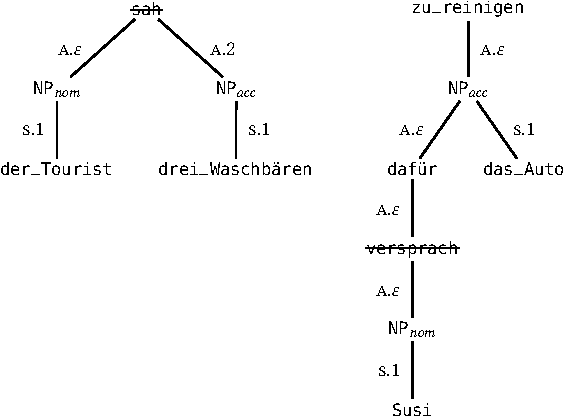
\includegraphics{graphics/abb826.pdf}
\caption{\label{fig-deanchoring-10}TT-MCTAG-Ableitungsbäume für das zweite Konjunkt in \ref{ex-deanchoring-8-a} und \ref{ex-deanchoring-8-b}}
\end{figure}
Ein \isi{A-Teilbaum} soll wieder ein maximaler Teilbaum des Ableitungsbaums\is{Ableitungsbaum} sein, der den \isi{Wurzelknoten} enthält und deren Kanten Adjunktionen\is{Adjunktion} repräsentieren, d.\,h.\ ein {\sc a}-Label besitzen.\footnote{Bei TT-MCTAG besteht außerdem die Möglichkeit, den \isi{A-Teilbaum}  anhand der benötigten Sharing-Lokalität weiter zu beschränken: Der A-Teilbaum besteht ausschlie\ss lich aus Knoten, die in einem Sharing-Verhältnis zum Wurzelknoten stehen. In den behandelten Fällen ist der Unterschied jedoch unwesentlich.} Beispielsweise bildet im linken Ableitungsbaum die Knotenmenge $\{${\tt sah}, {\tt NP\subnom}, {\tt NP\subacc}$\}$ den A-Teilbaum. Sei au\ss erdem ein \isi{S-Teilbaum} ein Teilbaum des Ableitungsbaums, dessen Wurzelknoten die S-Tochter eines Knotens des A-Teilbaums ist. Im linken Ableitungsbaum in Abbildung~\ref{fig-deanchoring-10} trifft das zum Beispiel auf die Knotenmengen $\{${\tt der\_Tourist}$\}$ und $\{${\tt drei\_Waschbären}$\}$ zu. Man stellt dann zunächst fest, dass (i) das finite Verb potentiell an beliebiger Position im A-Teilbaum stehen kann und (ii) die Knoten des A-Teilbaums beliebig entankert werden können -- mit Ausnahme des Knotens des finiten Verbs selbstverständlich. 

Die Gappingregeln\is{Gappingregel} G1--G3 (siehe Abschnitt~\ref{sec-gapping}) können folgenderma\ss en in den TT-MC\-TAG-Entankerungsansatz implementiert werden: 

\ex. {\bf Interne Bedingungen} (für das TT-MCTAG-Modell des Deutschen) \label{ex-interne-ttmctag}
\a. Falls ein Knoten im A-Teilbaum entankert wird, dann auch der Knoten des finiten Verbs im A-Teilbaum. ($\approx$ G1)\label{ex-interne-ttmctag-a}
\b. Falls ein Knoten $v$ im A-Teilbaum entankert wird, dann auch die Knoten all derjenigen S-Teilbäume, die $v$ unmittelbar dominiert. Falls ein Knoten in einem S-Teilbaum $\gamma$ entankert wird, dann werden alle Knoten in $\gamma$ entankert und derjenige Knoten im A-Teilbaum, der $\gamma$ unmittelbar dominiert. ($\approx$ G2)\label{ex-interne-ttmctag-b}
\c. Falls ein Knoten im A-Teilbaum entankert wird, dann auch der Knoten des \emph{dass}-Komplementierers im A-Teilbaum. ($\approx$~G3)\label{ex-interne-ttmctag-c}
\d. Mindestens ein Knoten des A-Teilbaums wird nicht entankert.\label{ex-interne-ttmctag-d} %($\approx$~G4)
 
Die G1-Implementierung\is{Gappingregel!G1} in \ref{ex-interne-ttmctag-a} setzt eine Identifizierbarkeit des finiten Verbs im A-Teil\-baum voraus. Das lässt sich leicht mit einem Merkmal, z.\,B.\ {\sc fin}, bewerkstelligen, welches finite Verben von infiniten Verben unterscheidet.\footnote{Es sei daran erinnert, dass es sich bei den Knotenlabeln um Merkmalsstrukturen handelt. Vgl.\ die Darstellung der partiellen Labelidentität in Abbildung~\ref{fig-deanchoring-9}.} Damit entsprechen sich \ref{ex-interne-ttmctag-a} und G1 auch insoweit, als beide für Ellipsemöglichkeiten in VE-Konfigurationen\is{Satz!VE-} noch zu restriktiv sind. Beispielsweise umfasst die Vorwärtsellipse\is{Ellipse!Vorwärts-} in \ref{ex-koord-8-a} auf Seite \pageref{ex-koord-8-a}, wiederholt in \ref{ex-koord-8-a-wdh}, nicht das finite Verb {\it erschoss}: 

\ex. \label{ex-koord-8-a-wdh}dass [$\kappa_1$ der Jäger den Hasen sah] und [$\kappa_1$ \sout{der Jäger} ihn erschoss].    

Der Ableitungsbaum bietet aber eigentlich alle Informationen, um dieses Ellipsenmuster zu lizenzieren: Man benötigt im Knoten des finiten Verbs nur ein zusätzliches Merkmal, das den Satztyp anzeigt. Da der Satztyp im TT-MCTAG-Modell immer durch den Elementarbaum des finiten Verbs festgelegt wird, ist diese Information an dieser Stelle auch immer verfügbar. Unter Einbezug dieses Satztypenmerkmals könnte die G1-Implementierung\is{Gappingregel!G1} in \ref{ex-interne-ttmctag-a} dann so umformuliert werden, dass sie nicht für VE-Satztypen gilt. Ich überspringe hier die Details. 

Die G2-Implementierung\is{Gappingregel!G2} in \ref{ex-interne-ttmctag-b} verhindert u.\,a.\ die partielle Ellipse des nominalen Satzglieds in \ref{ex-koord-17-b} auf Seite \pageref{ex-koord-17-b}, wiederholt in \ref{ex-koord-17-b-wdh}:

\ex. \#[$\kappa_1$ Der Jäger sah drei Hasen] und [$\kappa_2$ der Tourist \sout{sah drei} Waschbären].\label{ex-koord-17-b-wdh}

Die entsprechende Entankerung ist deshalb unzulässig, weil {\tt drei} und {\tt Waschbä\-ren} in jedem Fall Knoten eines S-Teilbaums\is{S-Teilbaum} sind, der nur im Ganzen entankert werden darf. Auf der  anderen Seite ist die G2-Implementierung permissiv genug, um Gapping in kohärenten Konstruktionen zu lizenzieren. Nehmen wir beispielsweise das Datum in \ref{ex-koord-21-a-wdh}, eine Wiederholung von \ref{ex-koord-21-a} auf Seite \pageref{ex-koord-21-a}, und den entsprechenden Ableitungsbaum in Abbildung~\ref{fig-deanchoring-koord-18}:

\ex. \label{ex-koord-21-a-wdh} [$\kappa_1$ Peter versprach, das Fahrrad zu reparieren] und [$\kappa_2$ Susi \sout{versprach} das Auto \sout{zu reparieren}].

\begin{figure}[t]
\centering
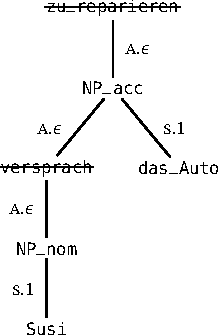
\includegraphics{graphics/abb827.pdf}
\caption{\label{fig-deanchoring-koord-18}TT-MCTAG-Ableitungsbäume für das zweite Konjunkt in \ref{ex-koord-21-a-wdh}}
\end{figure}
Dieses Entankerungsmuster ist deshalb möglich, weil gemä\ss\ \ref{ex-interne-ttmctag-b} die Knoten im \isi{A-Teilbaum} beliebig entankert werden können. Davon sind auch die Knoten des \isi{Verbalkomplex} betroffen, wodurch auch die Ellipsen in \ref{ex-koord-verbalkomplex-wdh}, eine Wiederholung von \ref{ex-koord-verbalkomplex} auf Seite \pageref{ex-koord-verbalkomplex}, derivierbar sind:  

\ex. [$\kappa_1$ Peter hat das Fahrrad zu reparieren versprochen]\label{ex-koord-verbalkomplex-wdh}
\a. und [$\kappa_2$ Susi \sout{hat das Fahrrad zu reparieren} versucht].
\b. ?und [$\kappa_2$ Susi \sout{hat das Fahrrad} zu benutzen \sout{versprochen}].\label{ex-koord-verbalkomplex-wdh-a}
\c. ??und [$\kappa_2$  Susi \sout{hat} das Auto \sout{zu reparieren} versucht].\label{ex-koord-verbalkomplex-wdh-b}

\largerpage
Will man jedoch, angesichts der fragwürdigen Grammatikalität von \ref{ex-koord-verbalkomplex-wdh-a} und \ref{ex-koord-verbalkomplex-wdh-b}, das Entankerungsverhalten so einschränken, dass der Verbalkomplex nur als Ganzes oder in einer bestimmten Reihenfolge entankert werden darf, dann bietet der Ableitungsbaum in dieser Form nicht die benötigten Unterscheidungen. Spezifische Entankerungsregeln für Verbalkomplexe kollidieren unweigerlich mit der freien Entankerbarkeit von A-Teilbaum-Knoten. Ähnlich wie bei der G1-Implementierung könnte man jedoch die Entankerbarkeit mittels spezieller Knotenmerkmale einschränken, die die Elemente des Verbalkomplexes für die Entankerungsregeln sichtbar machen. Prinzipiell stehen die dafür nötigen Informationen im Ableitungsbaum bzw.\ den zugrundeliegenden Elementarbäumen zur Verfügung.\is{Gappingregel!G2} 

Bisher habe ich \ref{ex-interne-ttmctag-b} als Implementierung von G2 bezeichnet und G2$^+$ in diesem Zusammenhang nicht erwähnt -- das hat einen guten Grund. G2$^+$\is{Gappingregel!G2$^+$} kommt bei der Lizenzierung satzübergreifenden Gappings\is{Ellipse!Gapping} wie in \ref{ex-koord-21-wdh}, eine Wiederholung von \ref{ex-koord-21-b} und \ref{ex-koord-21-c} auf Seite \pageref{ex-koord-21-b}, zum Tragen:
\largerpage%

\ex. \label{ex-koord-21-wdh}
\a. \label{ex-koord-21-b-wdh}[$\kappa_1$ Peter versprach, dass das Fahrrad repariert wird] und [$\kappa_2$ Susi \sout{versprach, dass} das Auto \sout{repariert wird}].
\b. \label{ex-koord-21-c-wdh}[$\kappa_1$ Peter freut sich, wenn das Fahrrad repariert wird], und [$\kappa_2$ Susi \sout{freut sich, wenn} das Auto \sout{repariert wird}].
 
Der Blick auf den fraglichen Ableitungsbaum in Abbildung~\ref{fig-deanchoring-11-2} offenbart nun, dass hier eine partielle Entankerung des S-Teilbaums unter {\tt repariert} erforderlich ist, die jedoch durch die zweite Klausel der internen Bedingungen blockiert wird. 
\begin{figure}[t]
\centering
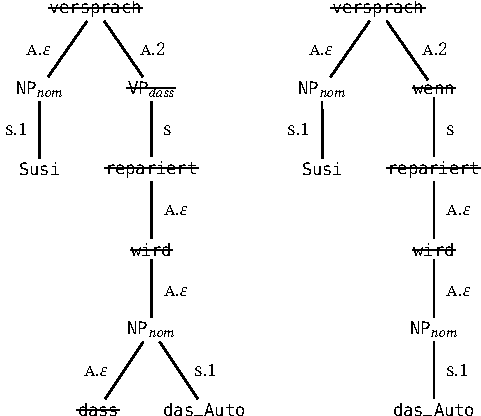
\includegraphics{graphics/abb828.pdf}
\caption{\label{fig-deanchoring-11-2}TT-MCTAG-Ableitungsbäume für die zweiten Konjunkte in \ref{ex-koord-21-b-wdh} und \ref{ex-koord-21-c-wdh}}
\end{figure}
Aus meiner Sicht sind drei Strategien vorstellbar, um G2$^+$\is{Gappingregel!G2$^+$}  zu implementieren: (i) man kann den Ableitungsbaum so verändern, dass die A-Teilbäume die richtige Grö\ss e erhalten; (ii) man kann die Definition der A-Teilbäume\is{A-Teilbaum} so anpassen, dass darin trotz Substitution auch die A-Teilbäume der Gliedsätze enthalten sind; (iii) man kann die Klausel \ref{ex-interne-ttmctag-b} so umformulieren, dass S-Teilbäume, die für bestimmte Teilsätze stehen, ausgenommen werden. Gehen wir diese Möglichkeiten im einzelnen durch:

\begin{itemize}
  \item Die Hineinsubstitutierung des {\it dass}-Komplementsatzes\is{Komplementsatz}\is{Satz!\textit{dass}-} ist aus Gründen der Lokalitätseinschränkung unumgänglich, denn TT-MCTAG definiert Bewegungsinseln\is{Bewegungsinsel} mittels der Substitution (siehe Abschnitt~\ref{sec-ttmctag-formalismus}). Würde also der {\it dass}-Komplementsatz\is{Komplementsatz} durch Adjunktion statt durch Substitution mit dem Matrixsatz verknüpft, so könnten die Ergänzungen von {\tt repariert} nicht nur unabhängig voneinander entankert, sondern auch au\ss erhalb des {\it dass}-Satzes platziert werden. Letzteres gilt es unbedingt zu vermeiden.\footnote{Dagegen kann bei V-TAG\is{Vector-MCTAG (V-TAG)} das Regens an einen {\it dass}-Komplementsatz\is{Komplementsatz} adjungieren, ohne dass gleichzeitig der Status als \isi{Bewegungsinsel} verloren geht. Bewegungsinseln werden bei V-TAG nämlich nicht durch Substitution, sondern durch beliebig auf Elementarbaumknoten platzierte Integrity Constraints\is{Integrity Constraint} hervorgerufen (siehe Abschnitt~\ref{sec-tag-varianten-vtag}). Damit würde wohl die ursprüngliche Formulierung der internen Bedingungen in \ref{ex-interne-ttmctag} ausreichen.}
  \item Die bessere Strategie scheint mir, die Definition der A-Teilbäume anzupassen: Ein \is{A-Teilbaum} $\gamma$ ist der maximale Teilbaum eines Ableitungsbaums $D$, so dass $\gamma$ ausschlie\ss lich den Wurzelknoten, Adjunktionskanten und solche Substitutionskanten, deren dominierender Knoten ein bestimmtes Label ({\tt VP\subelse{dass}}, {\tt wenn}, \ldots) oder Merkmal hat, umfasst. Strukturelle Kriterien, die sich allein auf die Verteilung von Adjunktions- und Substitutionskanten im Ableitungsbaum beziehen, reichen hier also nicht aus.%\footnote{Der Ansatz erinnert tatsächlich etwas an die Integrity Constraints bei V-TAG, nur dass hier ein Knoten markiert wird, in dessen dominierten Teilbaum ellidiert werden kann.}
  \item Statt die A-Teilbäume zu vergrö\ss ern, kann man auch die definitorische Bindung der A-Teilbäume an den Wurzelknoten des Ableitungsbaums aufheben, so dass ein Ableitungsbaum über mehr als einen \isi{A-Teilbaum} mit jeweils eigenen S-Teilbäumen verfügt. Dann lässt sich nämlich die b-Klausel in \ref{ex-interne-ttmctag} folgenderma\ss en umformulieren: (i) falls ein Knoten $v$ ohne ein bestimmtes Label ({\tt VP\subelse{dass}}, {\tt wenn}, \ldots) in einem A-Teilbaum $\gamma_a$ entankert wird, dann auch die Knoten all derjenigen S-Teilbäume, die $v$ unmittelbar dominiert; (ii) falls in einem \isi{S-Teilbaum} $\gamma_s$, der von einem Knoten $v'$ ohne ein bestimmtes Label ({\tt VP\subelse{dass}}, {\tt wenn}, \ldots) unmittelbar dominiert wird, ein Knoten entankert wird, dann werden $v'$ und alle Knoten in $\gamma_s$ entankert.  
\end{itemize} 
\newpage
Ich vermag nicht zu entscheiden, welche der letzten zwei Strategien die bessere ist. Erfreulich ist in jedem Fall, dass beide die Implementierung von G2$^+$\is{Gappingregel!G2$^+$} ermöglichen, ohne die Gestalt des Ableitungsbaums selber zu verändern. 

Weit weniger Aufwand verursacht die G3-Implementierung\is{Gappingregel!G3} in \ref{ex-interne-ttmctag-c}, die für die Blockierung von Daten wie \ref{ex-koord-6-c2-b-wdh}, das wir bereits in \ref{ex-koord-6-c2-b} auf Seite \pageref{ex-koord-6-c2-b} gesehen haben, zuständig ist: 

\ex. *[$\kappa_1$ Peter versprach, dass das Fahrrad repariert wird] und \newline [$\kappa_2$ Susi \sout{versprach}, dass das Auto \sout{repariert wird}].\label{ex-koord-6-c2-b-wdh}

Da der {\it dass}-Komplementierer\is{Komplementierer} im Ableitungsbaum per Knotenlabel leicht zu identifizieren ist, kann seine Entankerung ohne Weiteres durchgesetzt werden. 
\is{Entankerung!interne Bedingung für TT-MCTAG|)}


\subsection{Externe Bedingungen}\is{Entankerung!externe Bedingung für TT-MCTAG|(} 
	
Die externen Bedingungen aus \cite{Lichte:Kallmeyer:10}, die in \ref{ex-entankerung-externe-bedingungen} paraphrasiert wurden, fordern eine Pfadidentität und eine partielle Labelidentität zwischen entankerten Knoten und Antezedensknoten. Gilt das auch für den hier ausgearbeiteten TT-MCTAG-Entankerungs\-an\-satz? Nicht ganz. Aufgrund der Flexibilität der Wortstellung im Deutschen können sich Antezedenssatz\is{Antezedens} und Ellipsesatz in dieser Hinsicht unterscheiden: 

\ex. \label{ex-deanchoring-10}
\a. Den Gro\ss en nehme ich, und du \sout{nimmst} den Kleinen.\\ \citep[262]{Oirsouw:87}
\b. dass der Jäger einen Hasen sah und \sout{der Jäger} später drei Waschbären \sout{sah}.\label{ex-deanchoring-10-b}

Im TT-MCTAG-Modell geht die Wortstellungsdiskrepanz einher mit einer gewissen Strukturdiskrepanz in den involvierten Ableitungsbäume. Sichtbar wird das beispielsweise an den Ableitungsbäumen in Abbildung~\ref{fig-deanchoring-12} für die Konjunkte in Satz \ref{ex-deanchoring-10-b}. Die Knoten {\tt NP\subnom} und {\tt der\_Jäger} und ihre entankerten Gegenstücke haben jeweils einen anderen Pfad zum Wurzelknoten. Die Forderung nach der Identität der Pfade ist daher zu strikt. 
\begin{figure}[t]
\centering
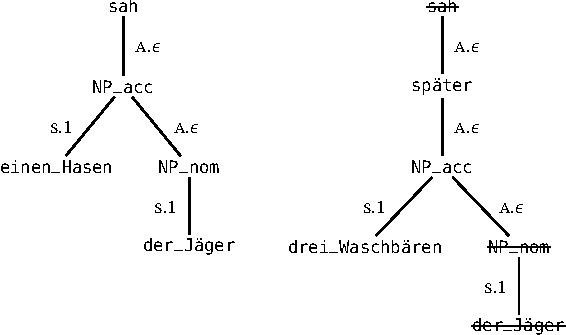
\includegraphics{graphics/abb829.pdf}
\caption{\label{fig-deanchoring-12}TT-MCTAG-Ableitungsbäume für die Konjunkte in \ref{ex-deanchoring-10}}
\end{figure}
Statt auf absoluter Pfadidentität muss im TT-MCTAG-Modell darauf gepocht werden, dass Ellipse- und Antezedensknoten entweder beide dem \isi{A-Teilbaum} im jeweiligen Ableitungsbaum oder beide den entsprechenden S-Teilbäumen\is{S-Teilbaum} angehören. Dabei ist zweierlei zu beachten: (i) innerhalb der S-Teilbäume (die ja nur vollständig entankert werden können) sollen Ellipse- und Antezedensknoten einen identischen Pfad zum jeweiligen Wurzelknoten haben, wobei (ii) entankerte S-Teilbäume genau einem S-Teilbaum im Antezedenssatz zugeordnet werden. Durch das Fehlen der absoluten Pfadidentität muss au\ss erdem explizit sichergestellt werden, dass das Abbildungsverhältnis von den entankerten Knoten auf deren Antezedensknoten injektiv ist, dass also kein Knoten im Antezedenssatz mehr als einen entankerten Knoten lizenziert. All dies wird in der folgenden Formulierung der externen Bedingungen berücksichtigt:  

\ex. {\bf Externe Bedingungen} (für das TT-MCTAG-Modell des Deutschen)
\a. Jeder entankerte Knoten hat genau einen Antezedensknoten und jeder Knoten des Ableitungsbaums des Antezedenssatzes lizenziert maximal einen entankerten Knoten.
\b. Ein entankerter Knoten und sein Antezedensknoten sind entweder Knoten des A-Teilbaums, oder sie sind Knoten mit identischem Pfad zum Wurzelknoten des jeweiligen S-Teilbaums, in dem sie sich befinden. (relative Pfadidentität) 
\c. Sei $v_{\mathit{ell}}$ ein entankerter Knoten und $\gamma_{\mathit{ell}}$ ein von $v_{\mathit{ell}}$ unmittelbar dominierter S-Teilbaum. Sei ferner $v_{\mathit{ant}}$ der Antezdensknoten von $v_{\mathit{ell}}$ und $\gamma_{\mathit{ant}}$ der von $v_{\mathit{ant}}$ unmittelbar dominierte S-Teilbaum. Es gilt dann: Alle Knoten in $\gamma_{\mathit{ell}}$ haben einen Antezedensknoten in $\gamma_{\mathit{ant}}$. 
\d. Ein entankerter Knoten und sein Antezdensknoten haben ein partiell identisches Knotenlabel. (partielle Labelidentität)   
 
Was die Labelidentität betrifft, so besteht kein Anlass zu wesentlichen Änderungen. Wie im Englischen können sich Ellipse und \isi{Antezedens} auch im Deutschen in manchen Aspekten unterscheiden (z.\,B.\ Numerus) und in anderen Aspekten müssen sie übereinstimmen (z.\,B.\ Tempus, vgl.\ \ref{ex-koord-23-a},~S.\,\pageref{ex-koord-23-a}, und \ref{ex-koord-24},~S.\,\pageref{ex-koord-24}):

\ex. 
\a. [$\kappa_1$ Gestern sah der Jäger einen Hasen] und [$\kappa_2$ die Touristen \sout{sahen} drei Waschbären].\label{ex-koord-23-a-wdh}
\b. \#[$\kappa_1$ Letztes Semester nahm Peter an einem Tanzkurs teil] und [$\kappa_2$ dieses Semester \sout{nimmt Peter} vielleicht auch \sout{an einem Tanzkurs teil}].\label{ex-koord-24-wdh}

Die partielle Identität komplexer Knotenlabel zu fordern, ist also auch hier angebracht.  %\\

Bevor ich diesen Abschnitt abschlie\ss e, sei noch darauf hingewiesen, dass sich der Entankerungsansatz auch auf Spinal-TT-MCTAG\is{TT-MCTAG!spinalisierte} anwenden lässt und die für TT-MCTAG gemachten Anpassungen im Wesenlichen auf Spinal-TT-MCTAG übertragen werden können. Dabei muss zwar auf die spezifische Form der Spinal-TT-MCTAG-Ableitungsbäume eingegangen werden, z.\,B.\ auf die Ent"-ankerung von Kettenelementen und die Entankerung der dazugehörigen S"=Teilbäumen. Es handelt sich aber in meinen Augen um rein technische Umformulierungen, die ich uns an dieser Stelle ersparen möchte. \\

\subsection{Zwischenstand}

\largerpage %long distance
In diesem Abschnitt habe ich zu zeigen versucht, wie die in Kapitel~\ref{chap-ellipse} identifizierten Gappingregeln\is{Gappingregel} in das TT-MCTAG-Modell aus Kapitel~\ref{sec-ttmctag} integriert werden können. Ich habe mich dabei auf die Formulierung der entsprechenden internen Bedingungen eines Entankerungsansatzes konzentriert. Sie lassen sich aber in trivialer Weise in die internen Bedingungen eines Füllungsansatzes\is{Füllung}, egal ob mit strukturierten oder unstrukturierten Füllungen, übertragen. Natürlich sind noch viele Detailfragen zu Modellierung und Implementierung offen, gerade was den Rekonstruktionsmachanismus betrifft, aber meiner Ansicht nach wird bereits deutlich, dass der Ableitungsbaum eine sehr nützliche Bezugsgrö\ss e für die Implementierung der Gappingregeln darstellt. 

Während also dieses erweiterte TT-MCTAG-Modell sowohl hinsichtlich kohärenter als auch hinsichtlich elliptischer Strukturen die gesteckten Ziele erreicht, ist die Asymmetrie seiner valenztheoretischen Fundierung auf"|fällig: Zwar wird die Idealisierung der Kontinuität weitgehend aufgegeben; die Idealisierung der Vollständigkeit\is{Idealisierung!der Vollständigkeit} bleibt aber bestehen -- erkennbar z.\,B.\ an den leeren Terminalen nach der Entankerung bzw.\ in den Dummy-Elementarbäumen. Daran ist zunächst nichts auszusetzen, da wir in erster Linie an der Möglichkeit einer Modellierung interessiert sind. In zweiter Linie interessiert uns aber natürlich auch, ob nicht auf die leeren Terminale irgendwie verzichtet werden kann und wie ein Syntaxmodell ohne Idealisierung der Vollständigkeit aussehen könnte. Wie wir im nächsten Abschnitt sehen werden, lässt sich erstere Frage auf einfache aber ebenso uninteressante Weise bejahen. Die Antwort auf die zweite Frage fällt dagegen weitaus schwerer und ist daher, wie so oft, spannender. Ihr ist daher zusätzlich das Kapitel~\ref{ch-ohne-valenz} gewidmet. 
\is{Entankerung!externe Bedingung für TT-MCTAG|)}


\section{Unvollständige syntaktische Repräsentation}\label{sec-unvollständige-repräsentation}\is{Unvollständigkeit}

Die Unvollständigkeit syntaktischer Repräsentation als Mittel der Ellipsenmodellierung kann im TAG-Framework sowohl im abgeleiteten Baum als auch im Ableitungsbaum in Erscheinung treten: Im abgeleiteten Baum bzw.\ in den Elementarbäumen fehlen diejenigen Blätter und im Ableitungsbaum diejenigen Knoten, die den ellidierten Valenzrahmenbestandteilen entsprechen. Gegen das TAG-Valenzprinzip (siehe S.\,\pageref{ex-valenzprinzip-tag}) muss hierbei selbstverständlich versto\ss en werden. Dies bedeutet jedoch nicht, dass die Unvollständigkeit im abgeleiteten Baum und Ableitungsbaum notwendigerweise zusammenfällt, denn zumindest bei der Gappingmodellierung kann der abgeleitete Baum unvollständig, der Ableitungsbaum jedoch vollständig sein. Dazu folgt gleich ein Beispiel. Und auch der skizzierte  Unvollständigkeitsbegriff ist keinesfalls monolithisch, denn er lässt eine Unterscheidung zwischen oberflächlichen und genuinen Unvollständigkeiten zu, die eine fundamentale Trennlinie definiert: die Trennlinie zwischen Syntaxkonzepten, denen der Valenzbezug inhärent ist, und Syntaxkonzepten, die nur einen indirekten Bezug zur Valenz haben.


\subsection{Oberflächliche Unvollständigkeit}\is{Unvollständigkeit!oberflächliche|(}

\largerpage%
Unter oberflächlicher Unvollständigkeit verstehe ich eine Form der Ellipsenmodellierung, bei der der Versto\ss\ gegen das Valenzprinzip\is{Wohlgeformtheitsprinzip!Valenzprinzip} als syntaktischer Spezialfall gilt und "`eigene syntaktische Regeln"' \citep{Klein:93} erfordert. Demgegenüber verkörpert die Wahrung des Valenzprinzips den Normalfall. Beispielsweise kann man, von einem vollständigen Elementarbaumschema für ditransitive Verben ausgehend, zusätzlich die unvollständigen Elementarbäume in Abbildung~\ref{fig-tag-unvoll-1} annehmen. In diese Richtung zielt auch der Vorschlag von \cite{Sarkar:97}, wobei dort je ein unvollständiger Elementarbaum mit einem vollständigen Gegenstück in einem 2-Tupel gebündelt und beide Elementarbäume für die synchrone Generierung der Konstituentenstruktur und der Dependenzstruktur\is{Dependenzgraph} eingesetzt werden.\footnote{Die 2-Tupel sind Elementarstrukturen einer sogenannten Link-Sharing TAG, wobei es sich, Sarkar zufolge, um eine etwas ausdrucksschwächere Variante einer synchronen TAG \citep{Shieber:Schabes:90} handelt.} 

\begin{figure}[t]
\centering
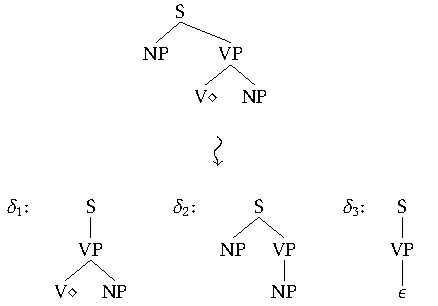
\includegraphics[angle=90]{graphics/abb830.pdf}
\caption{\label{fig-tag-unvoll-1}Unvollständige Elementarbaumschemata ($\delta_1$, $\delta_2$, $\delta_3$), die mit einem vollständigen Elementarbaum für ditransitive Verben korreliert sind}
\end{figure}

Mithilfe des unvollständigen Elementarbaums $\delta_2$ in Abbildung~\ref{fig-tag-unvoll-1} kann dann beispielsweise das Gappingexemplar in \ref{ex-unvoll-1} Ergebnis der Ableitung in Abbildung~\ref{fig-tag-unvoll-2} sein.

\ex. \label{ex-unvoll-1} Mary ate beans, and others \sout{ate} rice. %\hfill \citep{???}

\begin{figure}[t] 
\centering
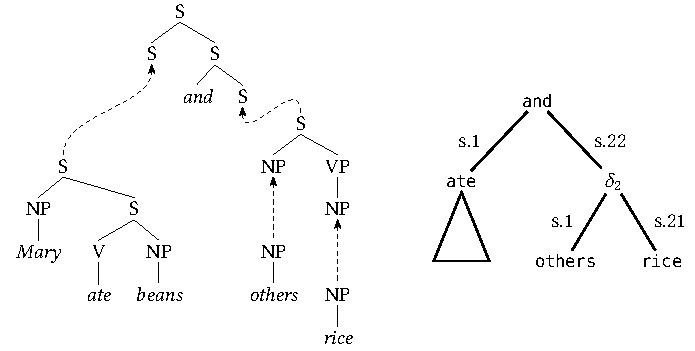
\includegraphics{graphics/abb831.pdf}
\caption{\label{fig-tag-unvoll-2}Gapping-Analyse mit dem unlexikalisierten Elementarbaum $\delta_2$}
\end{figure} 

Obwohl im abgeleiteten Baum die Strukturen des ellidierten Verbs fehlen, ist es im Ableitungsbaum weiterhin durch den Knoten $\delta_2$ syntaktisch repräsentiert. Wenn man also allein den Ableitungsbaum betrachtet, besteht kein wesentlicher Unterschied zum Füllungsansatz\is{Füllung} (vgl.\ Abbildung~\ref{fig-tag-fuellung-2}), denn die Struktur der Elementarbäume, abgesehen von nicht-terminalen Blättern, ist nur relevant für die Kombinatorik der Elementarbäume. Mit anderen Worten: Es spielt keine Rolle, ob beim Gapping das ellidierte Verb durch ein Dummy-Terminal im Elementarbaum repräsentiert wird, oder gar nicht wie bei $\delta_2$.\footnote{Während im TAG-Framework der Unterschied zwischen Füllung und oberflächlicher Unvollständigkeit marginal ist, kann er in Frameworks wie der \isi{GB-Theorie} oder HPSG\is{Head-driven Phrase Structure Grammar (HPSG)}, die sich an der abgeleiteten Struktur orientieren und über keine erweiterte Lokalitätsdomäne verfügen, wesentlich deutlicher ausfallen. Daher sind dort Vorschläge \`a la \cite{Chao:87} auch wesentlich interessanter. Vgl.\ Abschnitt~\ref{sec-ellipsenanalyse-wege}.}

Einen anderen Effekt hat dagegen die Verwendung der unvollständigen Elementarbäume $\delta_1$ und $\delta_3$. Da hier Substitutionsknoten für NP-Ergänzungen fehlen, fehlt auch deren Repräsentation als Knoten im Ableitungsbaum. Der Ableitungsbaum in Abbildung~\ref{fig-tag-unvoll-3} für die Subjektlücke\is{Ellipse!Subjektlücke} in \ref{ex-tag-unvoll-2} enthält also keinen Knoten, der dem ellidierten Subjekt entspricht:

\ex. \label{ex-tag-unvoll-2} Mary ate beans and \sout{Mary} drank wine.

\begin{figure}[t]
\centering
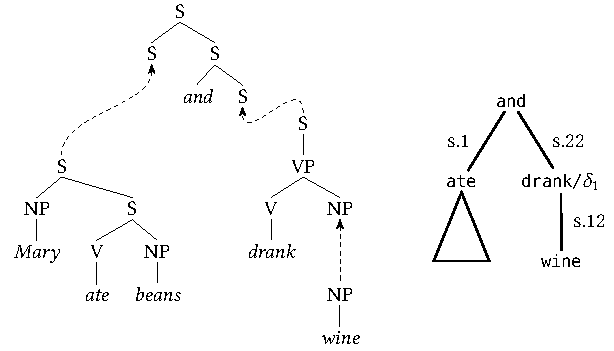
\includegraphics{graphics/abb832.pdf}
\caption{\label{fig-tag-unvoll-3}Derivation einer Subjektlücke mit dem unvollständigen Elementarbaum $\delta_1$}
\end{figure}
In gewisser Hinsicht ist hier also nicht nur der abgeleitete Baum, sondern auch der Ableitungsbaum unvollständig. Zwei Dinge gilt es jedoch zu beachten: (i) Der Eindruck ist falsch, dass zwischen der Unvollständigkeit des abgeleiteten Baums und des Ableitungsbaums ein bedingendes Verhältnis besteht. Der Elementarbaum für die Subjektlücke kann durchaus Dummy-Strukturen enthalten, die das ellidierte Subjekt repräsentieren sollen. (ii) Die Unvollständigkeit des Ableitungsbaums bezeichnet hier das Fehlen eines valenztheoretisch lizenzierten Blattes in einem Elementarbaum. Das bedeutet jedoch nicht, dass das ellidierte Subjekt gänzlich aus dem Ableitungsbaum verschwunden wäre. Es steckt quasi im Knotenlabel {\tt drank/$\delta_1$}, das eindeutig einen Elementarbaum mit Subjektlücke bezeichnet. 
\is{Unvollständigkeit!oberflächliche|)}




\subsection{Genuine Unvollständigkeit}\is{Unvollständigkeit!genuine|(}

Genuine Unvollständigkeit besteht dann, wenn die Verletzung gegen das Valenzprinzip\is{Wohlgeformtheitsprinzip!Valenzprinzip} kein Spezialfall der Syntax darstellt, wenn also die Ellipsenmodellierung keiner "`eigenen syntaktischen Regeln"' bedarf. In einem genuin unvollständigen TAG-Ansatz würde demnach kein Nebeneinander von unvollständigen und vollständigen Elementarbäume wie die in Abbildung~\ref{fig-tag-unvoll-2} bestehen. Als Folge dessen würde es auch nicht möglich sein, Hinweise auf eine Subjektlücke\is{Ellipse!Subjektlücke} in einem der Knoten des Ableitungsbaums vorzufinden, wie das mit {\tt drank/$\delta_1$} in Abbildung~\ref{fig-tag-unvoll-3} der Fall war. Das Fehlen des Subjekts müsste sich ausschlie\ss lich durch das Fehlen eines oder mehrerer Knoten im \isi{Ableitungsbaum} niederschlagen. 

Wie muss man sich eine TAG vorstellen, die solche Ableitungsbäume hat? Zwei Eigenschaften scheinen mir zentral: 
\begin{enumerate}
  \item Die Ergänzungen werden nicht durch nicht-terminale Blätter im Elementarbaum des Valenzträgers repräsentiert, denn sonst sind spezielle Elementarbäume für Vorfeldellipsen notwendig. Ergänzungen verhalten sich daher syntaktisch nicht anders als Angaben. 
  \item Die Elementarbäume der Ergänzungen eines Verbs können unabhängig vom Elementarbaum des Verbs in die Satzstruktur integriert werden, denn sonst muss für das Gapping\is{Ellipse!Gapping} ein spezieller Elementarbaum angenommen werden. Es besteht, mit anderen Worten, kein syntaktischer Verbzentrismus.
\end{enumerate}
Diese Eigenschaften hat beispielsweise die TAG-Analyse in Abbildung~\ref{fig-tag-unvoll-4}, wo spinalisierte Bäume mit der Fusionsoperation\is{Fusion} verknüpft werden. Spinalisierung und Fusion wurden bereits in Abschnitt \ref{sec-ttmctag-spinal} als Formalismuskomponenten der Spinal-TT-MCTAG\is{TT-MCTAG!spinalisierte} eingeführt. Im Unterschied zu einer Modellierung mit Spinal-TT-MCTAG sind die Elementarbäume in Abbildung~\ref{fig-tag-unvoll-4} aber nicht Bestandteile einer valenztheoretisch fundierten Multikomponentenstruktur. Tatsächlich wird hier das Valenzprinzip\is{Wohlgeformtheitsprinzip!Valenzprinzip} für Elementarstrukturen vollständig aufgegeben und es fehlt jeglicher Valenzbezug in der Syntax. 

\begin{figure}[t]
\centering
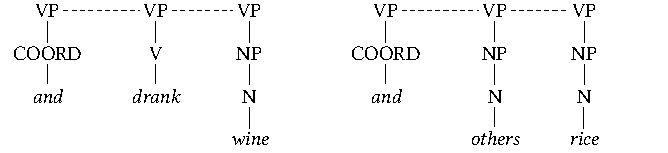
\includegraphics{graphics/abb833.pdf}
\caption{\label{fig-tag-unvoll-4}Genuin unvollständige Analyse der zweiten Konjunkte in \ref{ex-unvoll-1} und \ref{ex-tag-unvoll-2} mittels Fusion}
\end{figure}

Dieser TAG-Ansatz der genuinen Unvollständigkeit in der Ellipsenmodellierung und der daraus folgenden Abspaltung von Syntax und Valenz provoziert natürlich eine Reihe grundsätzlicher Fragen: 
\begin{itemize}
  \item Wie erfolgt hier das \isi{Argument Linking}?
  \item Was ist der dahinterstehende Syntax-Begriff? Ist er gerechtfertigt?
  \item Ist es gerechtfertigt, hier noch von einer TAG zu sprechen? Kann man sich nicht mit einem viel ausdrucksschwächeren Formalismus begnügen? 
  \item Was gewinnt man damit? Durch was rechtfertigt sich diese Abkehr vom Vertrauten, abgesehen vom Reiz des Neuen?
\end{itemize}
Angesichts dieser nicht einfach zu beantwortenden Fragen erstaunt es nicht, dass meines Wissens bisher noch kein Vorschlag in diese Richtung gemacht wurde, sei es im TAG-Framework oder im Rahmen irgendeines anderen Grammatikformalismus.\footnote{LTAG-spinal \citep{Shen:06,Shen:etal:08} verzichtet zwar auch weitgehend auf eine syntaktische Valenzrepräsentation, wird aber in erster Linie als ein Behelfsmittel für effizientes, inkrementelles LTAG-Parsen\is{Parsing} eingesetzt und nicht als linguistisches Modell.} Ich werde die Gelegenheit nutzen und im nächsten Kapitel die Perspektiven eines solchen Ansatzes umrei\ss en und seine Potentiale auszuloten versuchen. Dabei knüpfe ich an die Unterscheidung zwischen \isi{Phänogrammatik} und \isi{Tektogrammatik} zur Modellierung von kohärenten Konstruktionen und freier Wortstellung an, die in Abschnitt \ref{sec-kohaerenz-strategien-direkt} thematisiert wurden: Die Tektogrammatik, die Bezugsebene der Valenztheorie, ignoriert dann nicht nur die Kontinuität, sondern auch die Vollständigkeit der Valenzrahmenrealisierung.  
\is{Unvollständigkeit!genuine|)}



\section{Zusammenfassung}

In diesem Kapitel habe ich Modellierungsstrategien für elliptische Phänomene und ihre TAG-Umsetzungen dargestellt. Dem valenztheoretisch bestimmten Ellipsebegriff folgend orientiert sich die Taxonomie der Modellierungsstrategien an der vollständigen bzw.\ unvollständigen syntaktischen Repräsentation des Valenzrahmens. %Darin hebt sich unser Ansatz deutlich von anderen Taxonomien wie in \citet[5]{Winkler:Schwabe:03}, \citet[239f]{Culicover:Jackendoff:05}, \citet[2]{Aelbrecht:10} ab. 
Zu den Modellierungsstrategien, die von einer vollständigen syntaktischen Repräsentation des Valenzrahmens ausgehen, und damit von der Idealisierung der Vollständigkeit, zähle ich Reduktion, Verschmelzung und Füllung:
\begin{itemize}
  \item Bei der \textsc{Verschmelzung}\is{Verschmelzung} werden zwei valenztheoretisch vollständige syntaktische Strukturen kombiniert. Neben der Einschränkung, nur Koordinationsellipsen modellieren zu können, müssen auch hier zusätzliche Verknüpfungsoperationen ({\tt conjoin} bei \citealt{Sarkar:Joshi:96,Sarkar:Joshi:97}) bzw.\ der Versto\ss\ gegen das Valenzprinzip \citep{Seddah:08,Seddah:etal:10} in Kauf genommen werden. Zudem führen diese Ansätze eine massive lexikalische Ambiguität mit sich.  
  \item Die \textsc{Reduktion}\is{Reduktion} operiert auf bereits abgeleiteten, valenztheoretisch vollständigen, syntaktischen Strukturen und ersetzt Teile davon durch phonetisch leere Dummy-Elemente. Dazu zählt der Entankerungsansatz von \cite{Lichte:Kallmeyer:10}, der für ein LTAG-Fragment des Englischen entwickelt wurde. Ich konnte zeigen, dass die dortige Bezugnahme auf den Ableitungsbaum auch im TT"=MCTAG"=Modell des Deutschen als Werkzeug zur Generalisierung von Gappingmustern taugt. Wie die Entankerung im TAG"=Framework genau implementiert werden soll, ist jedoch noch offen.
  \item Bei einer \textsc{Füllung}\is{Füllung} flie\ss en die nicht realisierten Valenzrahmenbestandteile in Form von Dummy-Elementarbäumen in die syntaktische Ableitung ein. Dieses Vorgehen findet man bei \cite{Seddah:Sagot:06}. Eine gewisse Analogie zum Entankerungsansatz ist zu beobachten, die in der leichten Übertragbarkeit der internen Bedingungen auf dem Ableitungsbaum zum Ausdruck kommt. Allerdings stellt sich, zumindest bei strukturierten Füllungen, das Problem der massiven stringneutralen Übergenerierung. Eine enge derivationelle Verzahnung mit dem Antezedens scheint daher ratsam, muss aber noch genauer ausgearbeitet werden. 
\end{itemize}
Auch wenn gezeigt werden konnte, dass der Ableitungsbaum eine ausreichend informative Bezugsgröße bei der Implementierung von Reduktion und Füllung darstellt, ist damit natürlich noch nicht die eingangs gestellte Frage beantwortet, wie die Idealisierung der Vollständigkeit umgangen werden kann. Um darauf eine Antwort zu geben, habe ich mich zuletzt solchen Modellierungsstrategien zugewandt, die eine unvollständige syntaktische Repräsentation des Valenzrahmens ermöglichen. Eine wichtige Einsicht war hier, dass Unvollständigkeit in der Repräsentation nicht notwendigerweise mit einer fehlenden Idealisierung der Vollständigkeit einhergeht:
\begin{itemize}
  \item Als \textsc{oberflächlich unvollständig}\is{Unvollständigkeit!oberflächliche} bezeichne ich Ansätze, die zwar unvollständige Elementarstrukturen erlauben, diese aber speziell lizenzieren und interpretieren. Einen Vorschlag in diese Richtung macht \cite{Sarkar:97}. Abgesehen davon, dass hier weniger Struktur in den Elementarbäumen stipuliert wird und die Ableitungen in den Ableitungsbäumen kompakter repräsentiert werden können, besteht innerhalb des TAG-Frameworks kein wesentlicher Unterschied zu Füllungsansätzen mit unstrukturierten Füllungen.
\end{itemize}  
An die Stelle der weggelassenen Valenzrahmenbestandteile treten also syntaktische Kompensationsregeln. Dies gilt nicht nur für den TAG-Framework, sondern für alle hier untersuchten Frameworks mit irgendwie unvollständigen Repräsentationen. Der Weg führt also über den Ausschluss solcher Kompensationsregeln: 
\begin{itemize}   
  \item \textsc{Genuin unvollständig}\is{Unvollständigkeit!genuine} sind solche Ansätze, die unvollständige Valenzrealisierungen mittels Standardregeln modellieren. Das heißt mit anderen Worten, dass unvollständige Repräsentationen nicht als Spezialfall, sondern als Normalfall behandelt werden. 
\end{itemize}
Meines Wissens wurden genuin unvollständige Repräsentationen bei der Ellipsenmodellierung bisher noch nicht vorgeschlagen, geschweige denn detailliert ausgearbeitet. Das ist verständlich, wenn man sich die weitreichenden  Konsequenzen für die Grammatikarchitektur klar macht, nämlich das Verschwinden der valenzinduzierten  Trichotomie syntaktischer Einheiten (in \isi{Valenzträger}, \isi{Ergänzung} und \isi{Angabe}), und damit die Trennung von Syntax und Valenz. Es erscheint mir also nicht übertrieben, der Konkretisierung eines solchen Grammatikmodells das ganze nächste Kapitel zu widmen.



  